% !TEX root = ../popl-paper.tex

\begin{figure}[ht]
	\begin{center}
	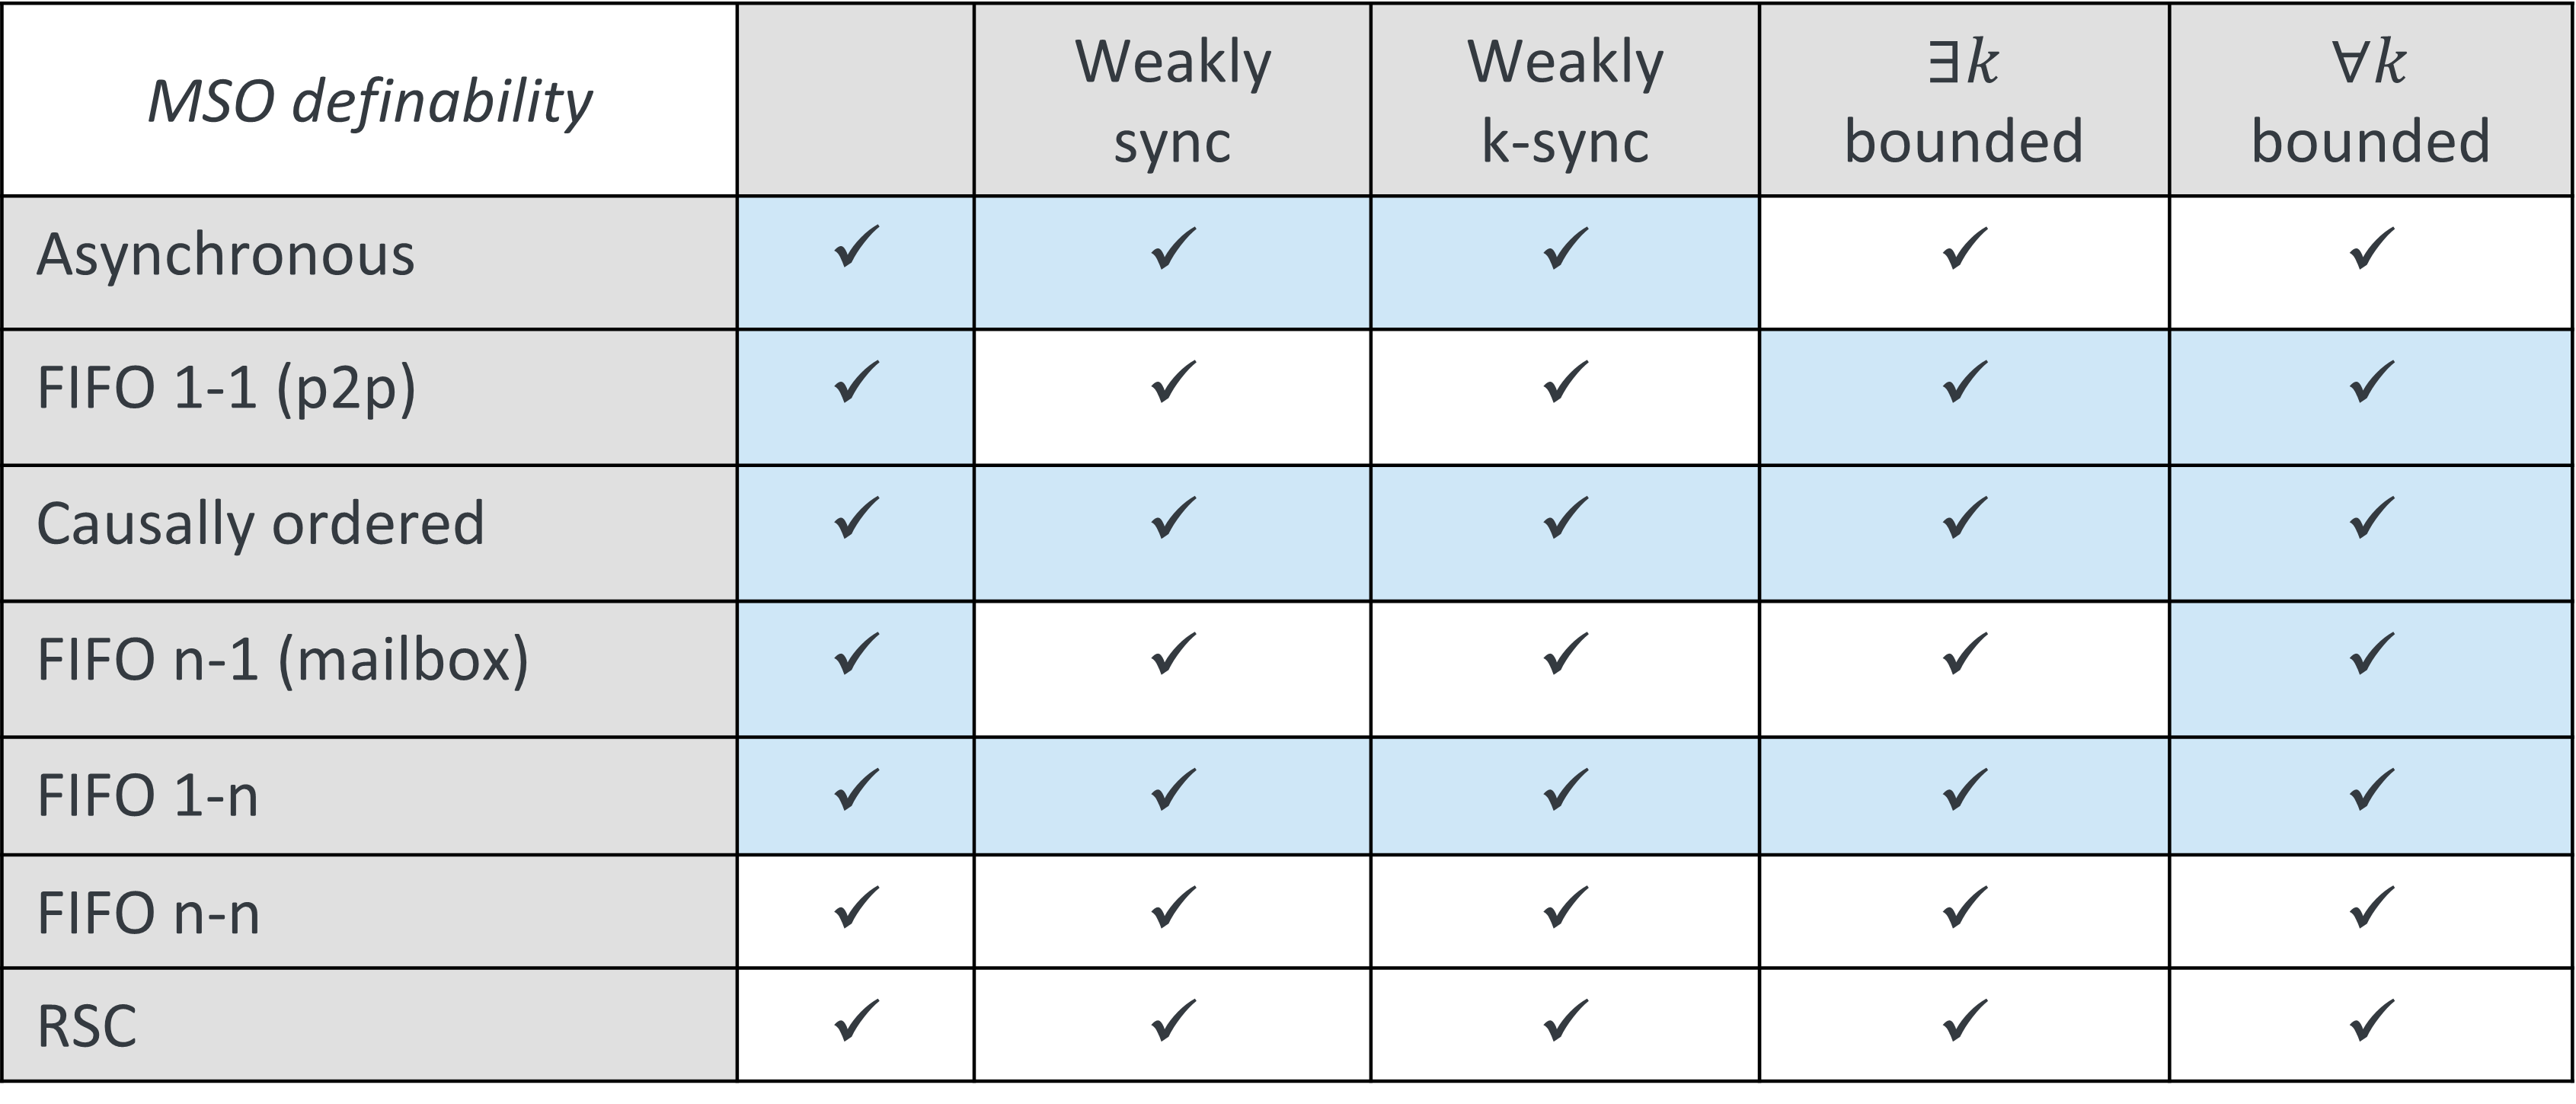
\includegraphics[width=10cm]{mso_def}
	\end{center}
\end{figure}

\begin{figure}[ht]
	\begin{center}
	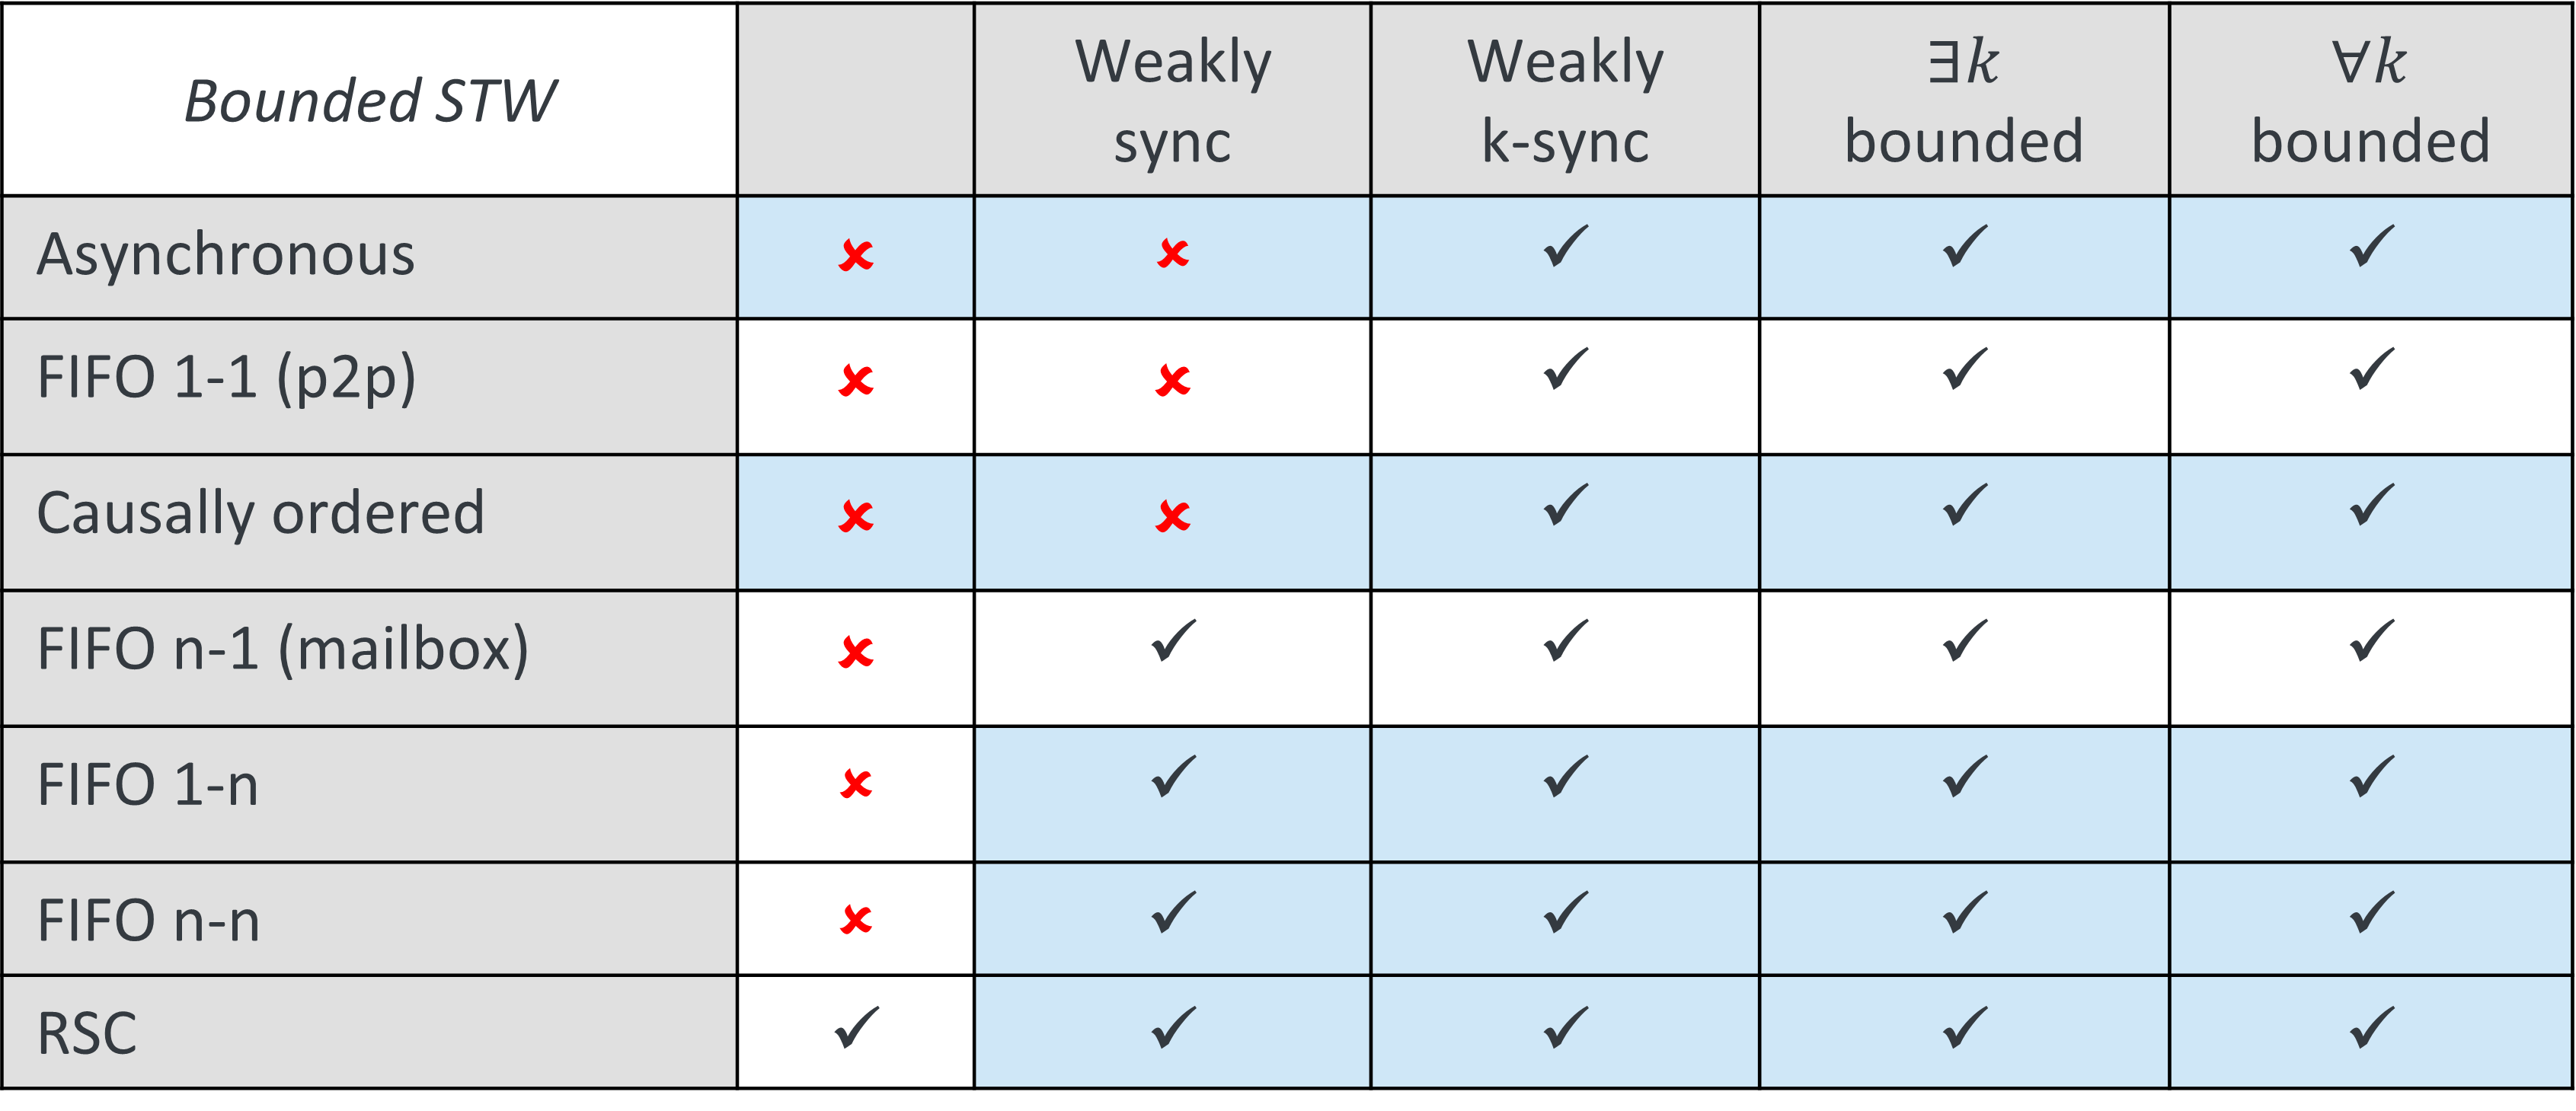
\includegraphics[width=10cm]{stw_bound}
	\end{center}
\end{figure}

% !TEX root = ../popl-paper.tex

\begin{figure}[t]
	\begin{center}
		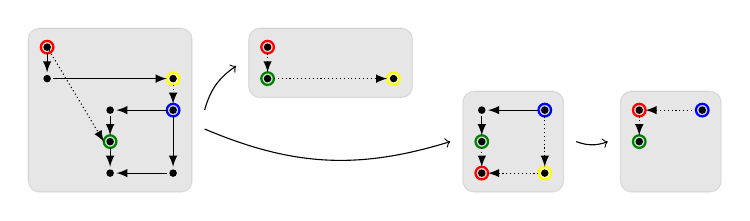
\begin{tikzpicture}[scale = .8]
			\begin{scope}
				\draw[gray,fill = gray, rounded corners, opacity=0.2] (-.3,.3) rectangle (2.3,-2.3);
				\draw[red, thick, fill = red!20] (0,0) circle (0.1);
				\draw[Green, thick, fill = Green!20] (1,-1.5) circle (0.1);
				\draw[Yellow, thick, fill = Yellow!20] (2,-.5) circle (0.1);
				\draw[blue, thick, fill = blue!20] (2,-1) circle (0.1);

				\draw[black, fill = black] (0,0) circle (.05);
				\draw[black, fill = black] (0,-.5) circle (.05);
				\draw[black, fill = black] (2,-.5) circle (.05);
				\draw[black, fill = black] (1,-1) circle (.05);
				\draw[black, fill = black] (2,-1) circle (.05);
				\draw[black, fill = black] (1,-1.5) circle (.05);
				\draw[black, fill = black] (1,-2) circle (.05);
				\draw[black, fill = black] (2,-2) circle (.05);

				\draw[>=latex, ->] (0,-.1) to (0, -.4);
				\draw[>=latex, ->,  densely dotted] (0,0) to (.9, -1.5);
				\draw[>=latex, ->] (.1,-.5) to (1.9, -.5);
				\draw[>=latex, ->,  densely dotted] (2,-.6) to (2, -.9);
				\draw[>=latex, ->] (1.9,-1) to (1.1, -1);
				\draw[>=latex, ->] (1,-1.1) to (1, -1.4);
				\draw[>=latex, ->] (1,-1.6) to (1, -1.9);
				\draw[>=latex, ->] (2,-1.1) to (2, -1.9);
				\draw[>=latex, ->] (1.9,-2) to (1.1, -2);

				\draw[->] (2.5,-1) to[bend left = 20] (3,-.3);
				\draw[->] (2.5,-1.3) to[bend right = 20] (6.4,-1.5);
				\draw[->] (8.4,-1.5) to[bend right = 20] (8.9,-1.5);


			\end{scope}
			\begin{scope}[shift = {(3.5,0)}]
				\draw[gray,fill = gray, rounded corners, opacity=0.2] (-.3,.3) rectangle (2.3,-.8);
				\draw[red, thick, fill = red!20] (0,0) circle (0.1);
				\draw[Green, thick, fill = Green!20] (0,-.5) circle (0.1);
				\draw[Yellow, thick, fill = Yellow!20] (2,-.5) circle (0.1);

				\draw[black, fill = black] (0,0) circle (.05);
				\draw[black, fill = black] (0,-.5) circle (.05);
				\draw[black, fill = black] (2,-.5) circle (.05);

				\draw[>=latex, ->, densely dotted	] (0,-.1) to (0, -.4);
				\draw[>=latex, ->, densely dotted	] (.1,-.5) to (1.9, -.5);
			\end{scope}
			\begin{scope}[shift = {(5.9,0)}]
				\draw[gray,fill = gray, rounded corners, opacity=0.2] (.7,-.7) rectangle (2.3,-2.3);
				\draw[red, thick, fill = red!20] (1,-2) circle (0.1);
				\draw[Green, thick, fill = Green!20] (1,-1.5) circle (0.1);
				\draw[Yellow, thick, fill = Yellow!20] (2,-2) circle (0.1);
				\draw[blue, thick, fill = blue!20] (2,-1) circle (0.1);

				\draw[black, fill = black] (1,-1) circle (.05);
				\draw[black, fill = black] (2,-1) circle (.05);
				\draw[black, fill = black] (1,-1.5) circle (.05);
				\draw[black, fill = black] (1,-2) circle (.05);
				\draw[black, fill = black] (2,-2) circle (.05);
				\draw[>=latex, ->] (1.9,-1) to (1.1, -1);
				\draw[>=latex, ->] (1,-1.1) to (1, -1.4);
				\draw[>=latex, ->,  densely dotted] (1,-1.6) to (1, -1.9);
				\draw[>=latex, ->,  densely dotted] (2,-1.1) to (2, -1.9);
				\draw[>=latex, ->,  densely dotted] (1.9,-2) to (1.1, -2);
			\end{scope}

			\begin{scope}[shift = {(8.4,0)}]
				\draw[gray,fill = gray, rounded corners, opacity=0.2] (.7,-.7) rectangle (2.3,-2.3);
				\draw[red, thick, fill = red!20] (1,-1) circle (0.1);
				\draw[Green, thick, fill = Green!20] (1,-1.5) circle (0.1);
				%\draw[Yellow, thick, fill = Yellow!20] (2,-2) circle (0.1);
				\draw[blue, thick, fill = blue!20] (2,-1) circle (0.1);

				\draw[black, fill = black] (1,-1) circle (.05);
				\draw[black, fill = black] (2,-1) circle (.05);
				\draw[black, fill = black] (1,-1.5) circle (.05);

				\draw[>=latex, ->,  densely dotted] (1.9,-1) to (1.1, -1);
				\draw[>=latex, ->,  densely dotted] (1,-1.1) to (1, -1.4);
				\end{scope}

		\end{tikzpicture}
	\end{center}
  \caption{Decomposition game for the MSC of Fig.~\ref{fig:pp_ex}. This is a 3-winning game for Eve.}
  \label{fig:stw-ex}
\end{figure}


In \cite{BolligFG21} the authors introduce a general framework based on MSO-logic and special treewidth that allows to derive decidability results for the \emph{synchronizability problem}. Roughly, the synchronizability problem consists in understanding whether all the behaviours/computations generated by a system have certain properties. The results in \cite{BolligFG21} hold for the $\oneone$ and the $\none$ communication models, which are referred to as p2p and mailbox, respectively. We show here that this framework can be effectively extended to all the 7 communication models that we considered.

%%%%%% COPY-PASTE from report

% \subsection{Semantics of causal ordering}

% \newcommand{\buffers}{\vv{\text{Buf}}}
% \newcommand{\clocks}{\vv{\text{Vec}}}
% \begin{definition}
% 	Given a system $\System = (Loc_p, \delta_p, \ell^0_p)_{p\in\procSet}$ with $n$ processes, a \emph{configuration} is a tuple $(\vv{\ell},\buffers,\clocks)$, where $\vv{\ell}=(\ell_p)_{p \in \procSet}$ represents the global state of the system, $\buffers=(b_p)_{p \in \procSet}$ is a vector of buffers, with each $b_p \in \Msg^*$ representing the content of the buffer of process $p$, and $\clocks=(v_p)_{p \in \procSet}$ is a vector of Mattern-Fidge logical clocks, where each $v_p = (time_i)_{i \in \procSet}$ represents the content of the logical vector clock of process $p$.
% \end{definition}

\subsection{Prefixes}

\begin{definition}[Prefix]
	Let $\msc = (\Events,\procrel,\lhd,\lambda) \in \MSCs$ and consider
	$E \subseteq \Events$ such that $E$ is ${\le_\msc}$-\emph{downward-closed}, i.e,
	for all $(e,f) \in {\le_\msc}$ such that $f \in E$, we also have $e \in E$.
	Then, the MSC $M' = (E,{\procrel} \cap (E \times E),{\lhd} \cap (E \times E),\lambda')$,
	where $\lambda'$ is the restriction of $\Events$ to $E$, is called a \emph{prefix}
	of $\msc$.
\end{definition}

If we consider a set $E$ that is ${\lessdot_\msc}$-\emph{downward-closed}, we call $M'$ a \emph{$\onen$ prefix}.
If the set $E$ is ${\bowtie_\msc}$-\emph{downward-closed}, we call $M'$ a \emph{$\nn$ prefix}. Note that every $\onen$ prefix and $\nn$ prefix is also a prefix, since $\le_\msc \subseteq {\lessdot_\msc}$ and $\le_\msc \subseteq {\bowtie_\msc}$.

Note that the empty MSC is a prefix of $\msc$.
We denote the set of prefixes of $\msc$ by $\Pref{\msc}$, whereas $\Prefonen{\msc}$ and $\Prefnn{\msc}$ are used for the $\onen$ and the $\nn$ variants, respectively.
This is extended to sets $L \subseteq \MSCs$ as expected, letting
$\Pref{L} = \bigcup_{\msc \in L} \Pref{\msc}$.

\begin{comment}

Let $\msc = (\Events,\procrel,\lhd,\lambda) \in \MSCs$ and consider
$E \subseteq \Events$ such that $E$ is ${\le_\msc}$-\emph{downward-closed}, i.e,
for all $(e,f) \in {\le_\msc}$ such that $f \in E$, we also have $e \in E$.
Then, the MSC $(E,{\procrel} \cap (E \times E),{\lhd} \cap (E \times E),\lambda')$,
where $\lambda'$ is the restriction of $\Events$ to $E$, is called a \emph{prefix}
of $\msc$. In particular, the empty MSC is a prefix of $\msc$.
We denote the set of prefixes of $\msc$ by $\Pref{\msc}$.
This is extended to sets $L \subseteq \MSCs$ as expected, letting
$\Pref{L} = \bigcup_{\msc \in L} \Pref{\msc}$.

\smallskip

Let $\msc = (\Events,\procrel,\lhd,\lambda) \in \onenMSCs$ and consider
$E \subseteq \Events$ such that $E$ is ${\lessdot_\msc}$-\emph{downward-closed}, i.e,
for all $(e,f) \in {\lessdot_\msc}$ such that $f \in E$, we also have $e \in E$.
Then, the MSC $(E,{\procrel} \cap (E \times E),{\lhd} \cap (E \times E),\lambda')$,
where $\lambda'$ is the restriction of $\Events$ to $E$, is called a \emph{$\onen$ prefix} of $\msc$. We denote the set of $\onen$ prefixes of $\msc$ by $\Prefonen{\msc}$.

\smallskip

Let $\msc = (\Events,\procrel,\lhd,\lambda) \in \nnMSCs$ and consider
$E \subseteq \Events$ such that $E$ is ${\bowtie_\msc}$-\emph{downward-closed}, i.e,
for all $(e,f) \in {\bowtie_\msc}$ such that $f \in E$, we also have $e \in E$.
Then, the MSC $(E,{\procrel} \cap (E \times E),{\lhd} \cap (E \times E),\lambda')$,
where $\lambda'$ is the restriction of $\Events$ to $E$, is called a \emph{$\nn$ prefix} of $\msc$. We denote the set of $\nn$ prefixes of $\msc$ by $\Prefnn{\msc}$.

\end{comment}

\subsection{Communicating Systems}

\begin{proposition}
	\label{prop:prefixes}
	For $\comsymb \in \{\asy, \oneone, \co, \none, \rsc\}$, every prefix of a $\comsymb$ MSC is a $\comsymb$ MSC.
\end{proposition}

Note that this proposition is not true for the $\onen$ and the $\nn$ communication models. Fig.\ref{fig:onen-prefix} shows an example of $\nn$ MSC with a prefix that is neither a $\nn$ MSC nor a $\onen$ MSC.

\begin{figure}[t]
	\captionsetup[subfigure]{justification=centering}
% \centering
\begin{subfigure}[t]{0.45\textwidth}\centering
	\begin{tikzpicture}[scale=0.7, every node/.style={transform shape}]
		\newproc{0}{p}{-1.5};
		\newproc{1}{q}{-1.5};
		\newproc{2}{r}{-1.5};

		\newmsgm{0}{1}{-0.5}{-0.5}{1}{0.3}{black};
		\newmsgm{0}{2}{-1.0}{-1.0}{2}{0.7}{black};

	\end{tikzpicture}
	\caption{A $\nn$ MSC $\msc$.}
\end{subfigure}
% \hfill
\begin{subfigure}[t]{0.45\textwidth}\centering
	\begin{tikzpicture}[scale=0.7, every node/.style={transform shape}]
		\newproc{0}{p}{-1.5};
		\newproc{1}{q}{-1.5};
		\newproc{2}{r}{-1.5};

		\newmsgum{0}{1}{-0.5}{1}{0.3}{black};
		\newmsgm{0}{2}{-1.0}{-1.0}{2}{0.7}{black};

	\end{tikzpicture}
	\caption{A prefix of $\msc$.}
\end{subfigure}
	\caption{A $\nn$ MSC with a prefix that is neither a $\onen$ MSC nor a $\nn$ MSC.}
	\label{fig:onen-prefix}
\end{figure}

\begin{proposition}
	\label{prop:prefixes-onen}
	Every $\onen$ prefix of a $\onen$ MSC is a $\onen$ MSC.
\end{proposition}
\begin{proposition}
	\label{prop:prefixes-nn}
	Every $\nn$ prefix of a $\nn$ MSC is a $\nn$ MSC.
\end{proposition}

\begin{comment}

\begin{lemma}
	\label{lem:p2p-prefix}
	Every prefix of a \pp MSC is a \pp MSC.
\end{lemma}
\begin{proof}
Let $\msc = (\Events, \procrel, \lhd, \lambda) \in \ppMSCs$ and let $\msc_0 =
(\Events_0, \procrel_0, \lhd_0, \lambda_0)$ be a prefix of $\msc$, where $\Events_0 \subseteq \Events$, ${\rightarrow_0} \subseteq {\rightarrow}$, and ${\lhd_0} \subseteq {\lhd}$. Since $\msc$ is \pp, we have that for every pair $(e,f) \in {\lhd}$, such that $\lambda(e) = \sact{p}{q}{\msg}$ and $\lambda(f) = \ract{p}{q}{\msg}$, $\sametype{e}{\pqsAct{p}{q}}{\procrel^+} = \sametype{f}{\pqrAct{p}{q}}{\procrel^+}$. We show that, for every pair $(e,f) \in {\lhd_0}$, this property still holds.
Since  ${\lhd_0} \subseteq {\lhd}$, every pair $(e,f)$ that belongs to $\lhd_0$ also belongs to $\lhd$, and we know that $\sametype{e}{\pqsAct{p}{q}}{\procrel^+} = \sametype{f}{\pqrAct{p}{q}}{\procrel^+}$.
Because of the $\le_\msc$-downward-closeness of $\Events_0$, it is easy to see that $\sametype{e}{\pqsAct{p}{q}}{\procrel^+}=\sametype{e}{\pqsAct{p}{q}}{\procrel_0^+}$ and $\sametype{f}{\pqrAct{p}{q}}{\procrel^+}=\sametype{f}{\pqrAct{p}{q}}{\procrel_0^+}$.
\end{proof}

\begin{lemma}
\label{lem:co-prefix}
Every prefix of a causally ordered MSC is a causally ordered MSC.
\end{lemma}
\begin{proof}
Let $\msc = (\Events, \procrel, \lhd, \lambda) \in \coMSCs$ and let $\msc_0 =
(\Events_0, \procrel_0, \lhd_0, \lambda_0)$ be a prefix of $\msc$. By contradiction, suppose that $\msc_0$ is not a	causally ordered MSC. There must be two distinct $s,s' \in \Events_0$ such that $\lambda(s)=\pqsAct{\plh}{q}$, $\lambda(s')=\pqsAct{\plh}{q}$, $s \le_{\msc_0} s'$ and either
\begin{enumerate*}[label={(\roman*)}]
	\item $r' \procrel^+ r$, where $r$ and $r'$ are two receive events such that $s \lhd r$ and $s' \lhd r'$, or
	\item $s \in \Unm{\msc_0}$ and $s' \in \Matched{\msc_0}$.
\end{enumerate*}
In both cases, $\msc$ would also not be a causally ordered $\MSCs$, since $\Events_0 \subseteq \Events$, ${\rightarrow_0} \subseteq {\rightarrow}$, and ${\lhd_0} \subseteq {\lhd}$. This is a contradiction, thus $\msc_0$ has to be causally ordered.
\end{proof}

\begin{lemma}
	\label{lem:onen-prefix}
	Every $\onen$ prefix of a $\onen$ MSC is a $\onen$ MSC.
\end{lemma}
\begin{proof}
	Let $\msc = (\Events, \procrel, \lhd, \lambda) \in \onenMSCs$ and let $\msc_0 =
	(\Events_0, \procrel_0, \lhd_0, \lambda_0)$ be a $\onen$ prefix of $\msc$, where $\Events_0 \subseteq \Events$. Firstly, the $\lessdot_\msc$-downward-closeness of $\Events_0$ guarantees that ${\msc_0}$ is still an MSC. We need to prove that it is a $\onen$ MSC. By contradiction, suppose that $\msc_0$ is not a $\onen$ MSC. Then, there are distinct $e,f \in \Events_0$ such that $e \lessdot_{\msc_0} f \lessdot_{\msc_0} e$, where $\lessdot_{\msc_0} = (\procrel_0 \cup \lhd_0 \cup \onenrel_{\msc_0})^\ast$. As $\Events_0 \subseteq \Events$, we have that ${\rightarrow_0} \subseteq {\rightarrow}$, ${\lhd_0} \subseteq {\lhd}$, ${\onenrel_{\msc_0}} \subseteq {\onenrel_\msc}$. Clearly, $\lessdot_{\msc_0} \subseteq \lessdot_\msc$, so $e \lessdot_\msc f \lessdot_\msc e$. This implies that $\msc$ is not a $\onen$ MSC, because $\lessdot_\msc$ is cyclic, which is a contradiction. Hence $\msc_0$ is a $\onen$ MSC.
\end{proof}

\noindent Note that every $\onen$ prefix is also a prefix.

\begin{lemma}
	\label{lem:nn-prefix}
	Every $\nn$ prefix of a $\nn$ MSC is a $\nn$ MSC.
\end{lemma}
\begin{proof}
	Let $\msc = (\Events, \procrel, \lhd, \lambda) \in \nnMSCs$ and let $\msc_0 =
	(\Events_0, \procrel_0, \lhd_0, \lambda_0)$ be a $\nn$ prefix of $\msc$, where $\Events_0 \subseteq \Events$. Firstly, the $\bowtie_\msc$-downward-closeness of $\Events_0$ guarantees that ${\msc_0}$ is still an MSC. We need to prove that it is a $\nn$ MSC. By contradiction, suppose that $\msc_0$ is not a $\nn$ MSC. Then, there are distinct $e,f \in \Events_0$ such that $e \bowtie_{\msc_0} f \bowtie_{\msc_0} e$. As $\Events_0 \subseteq \Events$, we have that ${\rightarrow_0} \subseteq {\rightarrow}$, ${\lhd_0} \subseteq {\lhd}$, ${\nnrel_0} \subseteq {\nnrel}$. Clearly, $\bowtie_{\msc_0} \subseteq\; \bowtie_\msc$, so $e \bowtie_\msc f \bowtie_\msc e$. This implies that $\msc$ is not a $\nn$ MSC, because $\bowtie_\msc$ is cyclic, which is a contradiction. Hence $\msc_0$ is a $\nn$ MSC.
\end{proof}

\noindent Note that every $\nn$ prefix is also a prefix.

\end{comment}

\begin{proposition}
	For all $\comsymb \in \{\oneone, \co, \none\}$, $\cL{\Sys}$ is prefix-closed:
	$\Pref{\cL{\Sys}} \subseteq \cL{\Sys}$.
\end{proposition}
\begin{proof}
	Follows from Lemma~\ref{lem:co-prefix}.
\end{proof}

\begin{proposition}
	$\onenL{\Sys}$ is $\onen$ prefix-closed:
	$\Prefonen{\onenL{\Sys}} \subseteq \onenL{\Sys}$.
\end{proposition}
\begin{proposition}
	$\nnL{\Sys}$ is $\nn$ prefix-closed:
	$\Prefnn{\nnL{\Sys}} \subseteq \nnL{\Sys}$.
\end{proposition}

\begin{comment}

Lemma~\ref{lem:prefix-closed} can be easily extendend to $\comsymb = \cosymb$.

\begin{lemma}\label{lem:co-prefix-closed}
	For all $\comsymb \in \{\ppsymb, \mbsymb, \cosymb\}$, $\cL{\Sys}$ is prefix-closed:
	$\Pref{\cL{\Sys}} \subseteq \cL{\Sys}$.
\end{lemma}
\begin{proof}
	Follows from Lemma~\ref{lem:co-prefix}.
\end{proof}

\begin{lemma}\label{lem:onen-prefix-closed}
	$\onenL{\Sys}$ is $\onen$ prefix-closed:
	$\Prefonen{\onenL{\Sys}} \subseteq \onenL{\Sys}$.
\end{lemma}
\begin{proof}
	Given a system $\System$, we have that $\onenL{\System} = \ppL{\System} \cap \onenMSCs$. Note that, because of how we defined a $\onen$ prefix, we have that $\Prefonen{\onenL{\Sys}} = \Pref{\onenL{\Sys}} \cap \onenMSCs$. Moreover, $\Pref{\onenL{\Sys}} \subseteq \Pref{\ppL{\Sys}}$, and $\Pref{\onenL{\Sys}} \subseteq \ppL{\Sys}$ for Lemma~\ref{lem:prefix-closed}. Putting everything together, $\Prefonen{\onenL{\Sys}} \subseteq \ppL{\Sys} \cap \onenMSCs = \onenL{\System}$.
\end{proof}

\begin{lemma}\label{lem:nn-prefix-closed}
	$\nnL{\Sys}$ is $\nn$ prefix-closed:
	$\Prefnn{\nnL{\Sys}} \subseteq \nnL{\Sys}$.
\end{lemma}
\begin{proof}
	Given a system $\System$, we have that $\nnL{\System} = \ppL{\System} \cap \nnMSCs$. Note that, because of how we defined a $\nn$ prefix, we have that $\Prefnn{\nnL{\Sys}} = \Pref{\nnL{\Sys}} \cap \nnMSCs$. Moreover, $\Pref{\nnL{\Sys}} \subseteq \Pref{\ppL{\Sys}}$, and $\Pref{\nnL{\Sys}} \subseteq \ppL{\Sys}$ for Lemma~\ref{lem:prefix-closed}. Putting everything together, $\Prefnn{\nnL{\Sys}} \subseteq \ppL{\Sys} \cap \nnMSCs = \nnL{\System}$.
\end{proof}

\end{comment}


\subsection{Model Checking}

\begin{theorem}
	\label{thm:bounded_model_checking}
	The bounded model-checking problem for $\comsymb \in \{$$\asy, $$\oneone, $$\co, $$\none, $$\onen, $$\nn, $$\rsc\}$ is decidable.
\end{theorem}

\begin{comment}

Knowing that $\coMSCs$ is MSO-definable, Theorem~\ref{thm:mailbox_bounded_model_checking} can be restated for $\comsymb = \cosymb$.

\begin{theorem}
	\label{thm:co_bounded_model_checking}
	The bounded model-checking problem for $\comsymb =  \cosymb$ is decidable.
\end{theorem}
\begin{proof}
By Proposition~\ref{prop:co_mso}, $\coMSCs=L(\coformula)$. Given a system $\System$, we have that $\coL{\System} = \ppL{\System} \cap L(\coformula)$. Therefore, we can rewrite the bounded model checking problem for $\comsymb = \cosymb$ as

\[\begin{array}{rl}
&\coL{\System} \cap \stwMSCs{k} \subseteq L(\phi)\\[1ex]
\Longleftrightarrow &\ppL{\System} \cap L(\coformula) \cap \stwMSCs{k} \subseteq L(\phi)\\[1ex]
\Longleftrightarrow &\ppL{\System} \cap \stwMSCs{k} \subseteq L(\phi) \cup L(\neg \coformula)\\[1ex]
\Longleftrightarrow &\ppL{\System} \cap \stwMSCs{k} \subseteq L(\phi \vee \neg \coformula)\,.
\end{array}\]
The latter is decidable due to Fact~\ref{p2p}.
\end{proof}

\begin{theorem}
	\label{thm:onen_bounded_model_checking}
	The bounded model-checking problem for $\comsymb =  \onensymb$ is decidable.
\end{theorem}
\begin{proof}
By Proposition~\ref{prop:onen_mso}, $\onenMSCs=L(\onenformula)$. Given a system $\System$, we have that $\onenL{\System} = \ppL{\System} \cap L(\onenformula)$. Therefore, we can rewrite the bounded model checking problem for $\comsymb = \onensymb$ as

\[\begin{array}{rl}
&\onenL{\System} \cap \stwMSCs{k} \subseteq L(\phi)\\[1ex]
\Longleftrightarrow &\ppL{\System} \cap L(\onenformula) \cap \stwMSCs{k} \subseteq L(\phi)\\[1ex]
\Longleftrightarrow &\ppL{\System} \cap \stwMSCs{k} \subseteq L(\phi) \cup L(\neg \onenformula)\\[1ex]
\Longleftrightarrow &\ppL{\System} \cap \stwMSCs{k} \subseteq L(\phi \vee \neg \onenformula)\,.
\end{array}\]
The latter is decidable due to Fact~\ref{p2p}.
\end{proof}

\begin{theorem}
	\label{thm:nn_bounded_model_checking}
	The bounded model-checking problem for $\comsymb =  \nnsymb$ is decidable.
\end{theorem}
\begin{proof}
By Proposition~\ref{prop:nn_mso}, $\nnMSCs=L(\nnformula)$. Given a system $\System$, we have that $\nnL{\System} = \ppL{\System} \cap L(\nnformula)$. Therefore, we can rewrite the bounded model checking problem for $\comsymb = \nnsymb$ as

\[\begin{array}{rl}
&\nnL{\System} \cap \stwMSCs{k} \subseteq L(\phi)\\[1ex]
\Longleftrightarrow &\ppL{\System} \cap L(\nnformula) \cap \stwMSCs{k} \subseteq L(\phi)\\[1ex]
\Longleftrightarrow &\ppL{\System} \cap \stwMSCs{k} \subseteq L(\phi) \cup L(\neg \nnformula)\\[1ex]
\Longleftrightarrow &\ppL{\System} \cap \stwMSCs{k} \subseteq L(\phi \vee \neg \nnformula)\,.
\end{array}\]
The latter is decidable due to Fact~\ref{p2p}.
\end{proof}

\end{comment}

\subsection{Synchronizability}

\begin{table}
	\centering
	\caption{Summary of the decidability of the synchronizability problem for different classes of MSCs.\label{table:my_summary}}
	\begin{adjustbox}{max width=\textwidth}
	\begin{tabular}{ |c||c|c|c| }
		\hline
		& \textsc{p2p}& \textsc{Causally ordered}& \textsc{Mailbox} \\
		\hline
		Weakly synchronous   & Undecidable [Thm.~\ref{thm:p2p-weak-sync}] & \textcolor{red}{Undecidable} [Thm.~\ref{thm:co-weak-sync}]   & EXPTIME [Thm.~\ref{thm:mailbox-weak-sync}] \\
		\hline
		Weakly $k$-synchronous &  \multicolumn{3}{c|} {\textcolor{red}{Decidable} [Thm.~\ref{thm:co-weak-k-sync}]}  \\
		\hline
		Existentially k-bounded & Decidable & \textcolor{red}{Decidable} & Decidable\\
		\hline
	\end{tabular}
	\end{adjustbox}
\end{table}

\begin{lemma}\label{lem:pref_stw_k+2}
	Let $k \in \N$ and $\Class \subseteq \stwMSCs{k}$. For all
	$M \in \MSCs \setminus \Class$, we have
	$(\Pref{\msc} \cap \stwMSCs{(k+2)}) \setminus \Class \neq \emptyset$.
\end{lemma}
\begin{proof}
	Let $k$ and $\Class$ be fixed, and let
	$\msc\in \MSCs\setminus \Class$ be fixed. If the empty MSC is not in $\Class$, then we are done, since it is a valid prefix of $\msc$ and it is in $\stwMSCs{(k+2)} \setminus \Class$.
	Otherwise, let $\msc'\in \Pref{\msc} \setminus \Class$ such that, for all $\le_\msc$-maximal events $e$ of $\msc'$, removing $e$ (along with its adjacent edges) gives an MSC in $\Class$. In other words, $\msc'$ is the "shortest" prefix of $\msc$ that is not in $\Class$. We obtain such an MSC by successively removing $\le_\msc$-maximal events. Let $e$ be $\le_{\msc'}$-maximal and let $\msc''=\msc' \setminus \{e\}$. Since $\msc'$ was taken minimal in terms of number of events,	$\msc''\in \Class$.
	So Eve has a winning strategy with $k+1$ pebbles for $\msc''$.
	Let us design a winning strategy with $k+3$ pebbles for Eve for $\msc'$, which will show the claim.

	Observe that the event $e$ occurs at the end of the timeline of a process (say $p$), and it is part of at most two edges:
	\begin{itemize}
		\item one with the previous $p$-event (if any)
		\item one with the corresponding send event (if $e$ is a receive event)
	\end{itemize}
	Let $e_1,e_2$ be the two neighbours of $e$.
	The strategy of Eve is the following: in the first round, mark $e,e_1,e_2$,
	then erase the edges $(e_1,e)$ and $(e_2,e)$, then split the remaining graph
	in two parts: $\msc''$ on the one side, and the single node graph $\{e\}$ on
	the other side. Then Eve applies its winning strategy for $\msc''$, except
	that initially the two events $e_1,e_2$ are marked (so she may need up to $k+3$
	pebbles).
\end{proof}

\begin{lemma}\label{lem:onen_pref_stw_k+2}
	Let $k \in \N$ and $\Class \subseteq \stwMSCs{k}$. For all
	$M \in \onenMSCs \setminus \Class$, we have
	$(\Prefonen{\msc} \cap \stwMSCs{(k+2)}) \setminus \Class \neq \emptyset$.
\end{lemma}
\begin{proof}
	Let $k$ and $\Class$ be fixed, and let
	$\msc\in \onenMSCs \setminus \Class$ be fixed. If the empty MSC is not in $\Class$, then we are done, since it is a valid $\onen$ prefix of $\msc$ and it is in $\stwMSCs{(k+2)} \setminus \Class$.
	Otherwise, let $\msc'\in \Prefonen{\msc} \setminus \Class$ such that, for all $\lessdot_\msc$-maximal events $e$ of $\msc'$, removing $e$ (along with its adjacent edges) gives an MSC in $\Class$. In other words, $\msc'$ is the "shortest" prefix of $\msc$ that is not in $\Class$. We obtain such an MSC by successively removing $\lessdot_\msc$-maximal events. Let $e$ be $\lessdot_{\msc'}$-maximal and let $\msc''=\msc' \setminus \{e\}$. Since $\msc'$ was taken minimal in terms of number of events,	$\msc''\in \Class$.
	The proof proceeds exactly as the proof of Lemma~\ref{lem:pref_stw_k+2}.
\end{proof}

\begin{lemma}\label{lem:nn_pref_stw_k+2}
	Let $k \in \N$ and $\Class \subseteq \stwMSCs{k}$. For all
	$M \in \nnMSCs \setminus \Class$, we have
	$(\Prefnn{\msc} \cap \stwMSCs{(k+2)}) \setminus \Class \neq \emptyset$.
\end{lemma}
\begin{proof}
	Let $k$ and $\Class$ be fixed, and let
	$\msc\in \nnMSCs \setminus \Class$ be fixed. If the empty MSC is not in $\Class$, then we are done, since it is a valid $\nn$ prefix of $\msc$ and it is in $\stwMSCs{(k+2)} \setminus \Class$.
	Otherwise, let $\msc'\in \Prefnn{\msc} \setminus \Class$ such that, for all $\bowtie_\msc$-maximal events $e$ of $\msc'$, removing $e$ (along with its adjacent edges) gives an MSC in $\Class$. In other words, $\msc'$ is the "shortest" prefix of $\msc$ that is not in $\Class$. We obtain such an MSC by successively removing $\bowtie_\msc$-maximal events. Let $e$ be $\bowtie_{\msc'}$-maximal and let $\msc''=\msc' \setminus \{e\}$. Since $\msc'$ was taken minimal in terms of number of events,	$\msc''\in \Class$.
	The proof proceeds exactly as the proof of Lemma~\ref{lem:pref_stw_k+2}.
\end{proof}

Note that Lemma~\ref{lem:continuous} can be extended to $\comsymb = \cosymb$, since Lemma~\ref{lem:continuous2} does not depend on the kind of communication used by the system.

\begin{lemma}\label{lem:continuous_co}
Let $\System$ be a communicating system, $\comsymb \in \{\ppsymb, \mbsymb, \cosymb\}$,
$k \in \N$, and $\Class \subseteq \stwMSCs{k}$.
Then, $\cL{\System} \subseteq \Class$ iff
$\cL{\System} \cap \stwMSCs{(k+2)} \subseteq \Class$.
\end{lemma}

\begin{lemma}\label{lem:continuous_onen}
Let $\System$ be a communicating system,
$k \in \N$, and $\Class \subseteq \stwMSCs{k}$.
Then, $\onenL{\System} \subseteq \Class$ iff
$\onenL{\System} \cap \stwMSCs{(k+2)} \subseteq \Class$.
\end{lemma}
\begin{proof}
	Follows from Lemma~\ref{lem:onen-prefix-closed} and Lemma~\ref{lem:onen_pref_stw_k+2}.
\end{proof}

\begin{lemma}\label{lem:continuous_nn}
Let $\System$ be a communicating system,
$k \in \N$, and $\Class \subseteq \stwMSCs{k}$.
Then, $\nnL{\System} \subseteq \Class$ iff
$\nnL{\System} \cap \stwMSCs{(k+2)} \subseteq \Class$.
\end{lemma}
\begin{proof}
	Follows from Lemma~\ref{lem:nn-prefix-closed} and Lemma~\ref{lem:nn_pref_stw_k+2}.
\end{proof}

Theorem~\ref{thm:sync} can also be extended to $\comsymb = \cosymb$.

\begin{theorem}\label{thm:sync_co}
Fix finite sets $\Procs$ and $\Msg$.
Suppose $\comsymb \in \{\ppsymb, \mbsymb,\cosymb\}$ and let $\Class \subseteq \MSCs$ be an MSO-definable and STW-bounded class (over $\Procs$ and $\Msg$).
The following problem is decidable:
Given a communicating system $\System$, do we have $\cL{\System} \subseteq \Class$?
\end{theorem}
\begin{proof}
Same as the proof for Theorem~\ref{thm:sync}, but using Lemma~\ref{lem:continuous_co} in place of Lemma~\ref{lem:continuous}, and Theorem~\ref{thm:co_bounded_model_checking} in place of Theorem~\ref{thm:mailbox_bounded_model_checking}.
\end{proof}

\begin{theorem}\label{thm:sync_onen}
Fix finite sets $\Procs$ and $\Msg$.
Let $\Class \subseteq \MSCs$ be an MSO-definable and STW-bounded class (over $\Procs$ and $\Msg$).
The following problem is decidable:
Given a communicating system $\System$, do we have $\onenL{\System} \subseteq \Class$?
\end{theorem}
\begin{proof}
Same as the proof for Theorem~\ref{thm:sync}, but using Lemma~\ref{lem:continuous_onen} in place of Lemma~\ref{lem:continuous}, and Theorem~\ref{thm:onen_bounded_model_checking} in place of Theorem~\ref{thm:mailbox_bounded_model_checking}.
\end{proof}

\begin{theorem}\label{thm:sync_nn}
	Fix finite sets $\Procs$ and $\Msg$.
	Let $\Class \subseteq \MSCs$ be an MSO-definable and STW-bounded class (over $\Procs$ and $\Msg$).
	The following problem is decidable:
	Given a communicating system $\System$, do we have $\nnL{\System} \subseteq \Class$?
	\end{theorem}
\begin{proof}
Same as the proof for Theorem~\ref{thm:sync}, but using Lemma~\ref{lem:continuous_nn} in place of Lemma~\ref{lem:continuous}, and Theorem~\ref{thm:nn_bounded_model_checking} in place of Theorem~\ref{thm:mailbox_bounded_model_checking}.
\end{proof}

\subsubsection{Weakly synchronous causally ordered MSCs}

Corollary~\ref{cor:weak-sync-lcpdl} can  be extended to $\comsymb = \cosymb$.

\begin{proposition}\label{cor:co-weak-sync-mso}
The set of weakly synchronous \emph{causally ordered} MSCs is MSO-definable.
\end{proposition}
\begin{proof}
Both the sets of weakly synchronous MSCs and of causally ordered MSCs are MSO-definable, as shown by Corollary~\ref{cor:weak-sync-lcpdl} and Proposition~\ref{prop:co_mso}. Recall that any LCPDL-definable property is also MSO-definable. It suffices to take the conjuction of the two respective MSO formulas.
\end{proof}

\begin{theorem}\label{thm:co-weak-sync}
The following problem is undecidable:
Given finite sets $\Procs$ and $\Msg$ as well as a communicating system $\System$,
is every MSC in $\coL{\System}$ weakly synchronous?
\end{theorem}
\begin{proof}
The proof is essentially identical to the \pp case. We do the same reduction from the Post correspondence problem. Recall from the proof of Theorem~\ref{thm:p2p-weak-sync} that we consider a system $\System$ with four machines (P1, P2, V1, V2), where we have unidirectional communication channels from provers to verifiers. In particular notice that all the possible behaviours of $\System$ are causally ordered, i.e. $\ppL{\System} \subseteq \coMSCs$; according to how we built our system $\System$, it is impossible to have a pair of causally-related send events of P1 and P2\footnote{There is no channel between P1 and P2, and we only have unidirectional communication channels from provers to verifiers; it is impossible to have a causal path between two send events of P1 and P2.}, which implies that causal ordering is already ensured by any possible \pp behaviour of $\System$. The rest of the proof is identical to the \pp case.
\end{proof}

\begin{corollary}
The set of weakly synchronous causally ordered MSCs has unbounded special tree-width.
\end{corollary}
\begin{proof}
Suppose that the set of weakly synchronous causally ordered MSCs is STW-bounded. By Proposition \ref{cor:co-weak-sync-mso} and Theorem~\ref{thm:sync_co}, we have that the syncronicity problem for the class of weakly synchronous causally ordered MSCs would be decidable. This is a contradiction, since Theorem~\ref{thm:co-weak-sync} states that this problem is undecidable.
\end{proof}

\subsubsection{Weakly \texorpdfstring{$k$}{k}-synchronous causally ordered MSCs}

\begin{proposition}\label{prop:co-weak-k-sync-mso}
The set of weakly \emph{k}-synchronous causally ordered MSCs is MSO-definable.
\end{proposition}
\begin{proof}
Both the sets of weakly \emph{k}-synchronous MSCs and of causally ordered MSCs are MSO-definable, as shown by Proposition~\ref{prop:weak-logic-bounded} and Proposition~\ref{prop:co_mso}. It suffices to take the conjuction of the two respective MSO formulas.
\end{proof}

% Note that every causally ordered \emph{k}-synchronous MSC is also a  $\ppsymb$ \emph{k}-synchronous MSC.
Theorem~\ref{thm:sync} can be easily extended to $\comsymb = \cosymb$.

\begin{theorem}\label{thm:co-weak-k-sync}
For $\comsymb \in \{\ppsymb, \mbsymb,\cosymb\}$, the following problem is decidable:
Given finite sets $\Procs$ and $\Msg$, a communicating system $\System$, and $k \in \N$,
is every MSC in $\cL{\System}$ weakly $k$-synchronous?
\end{theorem}
\begin{proof}
By Proposition~\ref{prop:co-weak-k-sync-mso} and Proposition~\ref{prop:kweakstw} we have that the class of causally ordered \emph{k}-synchronous MSCs is MSO-definable and STW-bounded\footnote{Note that Proposition~\ref{prop:kweakstw} is independent from the type of communication.}. Theorem~\ref{thm:sync_co} ends the proof.
\end{proof}

\subsubsection{Existentially \texorpdfstring{$k$}{k} causally ordered bounded MSCs}

\begin{definition}
Let $\msc = (\Events,\procrel,\lhd,\lambda) \in \MSCs$ and $k \in \N$.
A linearization $\linrel$ of $\msc$ is called
$k$-\emph{bounded} if, for all $e \in \Matched{\msc}$, with $\lambda(e) = \sact{p}{q}{\msg}$, we have
\[
\sametype{e}{\pqsAct{p}{q}}{\linrel} - \sametype{e}{\pqrAct{p}{q}}{\linrel} \le k.
\]
\end{definition}
\noindent Recall that $\sametype{e}{\pqsAct{p}{q}}{\linrel}$ denotes the number of send events from $p$ to $q$ that occured before $e$, according to $\linrel$.

\begin{definition}\label{def:ex_k_pp_bounded}
	An MSC is said to be \emph{existentially \pp bounded} ($\exists k$-$\pp$-bounded) if it has a $k$-bounded linearization.
\end{definition}

\begin{definition}\label{def:ex_k_co_bounded}
An MSC is said to be \emph{existentially $k$ causally ordered bounded} ($\exists k$-$\cosymb$-bounded) if it is causally ordered and it has a $k$-bounded linearization.
\end{definition}

Note that every existentially $k$ causally ordered bounded MSC is an existentially $k$-\pp-bounded MSC.

\begin{proposition}\label{prop:ek-co-bounded-mso-stw}
For all $k \in \N$, the set of $\exists k$-$\cosymb$-bounded MSCs is MSO-definable and STW-bounded.
\end{proposition}
\begin{proof}
Let $\ppEk$ and $\coEk$ be the set of existentially $k$-\pp-bounded MSCs and the set of existentially $k$ causally ordered bounded MSCs, respectively. $\ppEk$ was shown to be both MSO-definable (in \cite{DBLP:journals/iandc/LohreyM04}) and STW-bounded (in \cite[Proposition 5.4, page 163]{DBLP:journals/corr/abs-1904-06942}). $\coEk$ also has to be STW-bounded, since we have $\coEk \subseteq \ppEk$. Note that, by definition, $\coEk = \ppEk\, \cap\, \coMSCs$. Since both $\ppEk$ and $\coMSCs$ can be defined by an MSO formula, the latter according to Proposition~\ref{prop:co_mso}, $\coEk$ is also MSO-definable\footnote{Suppose $\varphi_{\exists k\text{-}\pp\text{-}b}$ is the MSO formula for $\ppEk$, and $\coformula$ is the MSO formula for $\coMSCs$. Then, $\coEk$ is defined by $\varphi_{\exists k\text{-}\cosymb\text{-}b} = \varphi_{\exists k\text{-}\pp\text{-}b} \wedge \coformula$}.
\end{proof}

\begin{theorem}\label{thm:sync_ek_co_bounded}
	The following problem is decidable: Given finite sets $\Procs$ and $\Msg$, a communicating system $\System$, and $k \in \N$, is every MSC in $\coL{\System}$ $\exists k$-$\cosymb$-bounded?
\end{theorem}
\begin{proof}
	Directly follows from \ref{prop:ek-co-bounded-mso-stw} and \ref{thm:sync_co}.
\end{proof}

\subsection{Monadic Second-Order Logic}

The set of MSO formulas over (asynchronous) MSCs (over $\Procs$ and $\Msg$) is given by the grammar
$
\phi ::= true \mid x \procrel y \mid x \lhd y \mid \lambda(x) = a \mid x = y \mid x \in X \mid \exists x.\phi \mid \exists X.\phi \mid \phi \vee \phi \mid \neg \phi
$,
where $a \in \Act$, $x$ and $y$ are first-order variables, interpreted as
events of an MSC, and $X$ is a second-order variable, interpreted
as a set of events. We assume that we have an infinite supply of variables,
and we use common abbreviations such as $\wedge$, $\Rightarrow$, $\forall$, etc.
The satisfaction relation is defined in the standard way and self-explanatory.
For example, the formula $\neg\exists x.(\bigvee_{a \in \sAct} \lambda(x) = a \;\wedge\; \neg \mathit{matched}(x))$
with $\mathit{matched}(x) = \exists y.x \lhd y$
says that there are no unmatched send events.
It is not satisfied by  MSC $\mscweakuniver$
of Fig.~\ref{fig:msc_weak_univer},
as message $\msg_1$ is not received,
but by $\mscstrongexist$ from Fig.~\ref{fig:msc_strong_exist}.

Given a sentence $\phi$, i.e., a formula without free variables,
we let $L(\phi)$ denote the set of MSCs that satisfy $\phi$. Since we have defined the set of MSO formulas over asynchronous MSCs, the formula $\asformula = true$ clearly describes the set of asynchronous MSCs, i.e. $L(\asformula) = \asMSCs$. It is worth mentioning that the (reflexive) transitive closure of a binary relation defined by an MSO formula\footnote{See Section~\ref{sec:mso_extra} for details.} with free variables $x$ and $y$, such as $x \procrel y$, is MSO-definable so that the logic can freely use formulas of the form $x \procrel^+ y$, $x \procrel^* y$ or $x \le y$ (where $\le$ is interpreted as $\le_\msc$ for the given MSC $\msc$).

\paragraph*{Peer-to-peer MSCs}
	The set of \pp MSCs is MSO-definable as
	\[
		\ppformula = \neg \exists s.\exists s'. \left(
		\bigvee_{\substack{p \in \Procs, q \in \Procs}}\;
		\bigvee_{\substack{a,b \in \pqsAct{p}{q}}}\hspace{-1em}
		(\lambda(s) = a \;\wedge\; \lambda(s') = b) \;\wedge\; s \procrel^+ s' \;\wedge\;
		(\psi_1 \vee \psi_2 )
		\right)
	\]
	where $\psi_1$ and $\psi_2$ are
	\[
		\psi_1 = \exists r.\exists r'.\left(
		\begin{array}{ll}
			s \lhd r & \wedge\\
			s' \lhd r' & \wedge\\
			r' \procrel^+ r &
		\end{array}
		\right) \quad \quad
		\psi_2 = (\neg \mathit{matched}(s) \wedge \mathit{matched}(s'))
		\]
		\[
		matched(x) = \exists y. x \lhd y
	\]

The property $\ppformula$ says that there cannot be two matched send events $s$ and $s'$, with the same sender and receiver, such that either
\begin{enumerate*}[label={(\roman*)}]
	\item $s \procrel^+ s'$ and their receipts happen in the reverse order, or
	\item $s$ is unmatched and $s'$ is matched.
\end{enumerate*}
In other words, it ensures that channels operate in FIFO mode, where an unmatched messages blocks the receipt of all the subsequent messages on that channel.
The set $\ppMSCs$ is therefore MSO-definable as $\ppMSCs=L(\ppformula)$.

\paragraph*{Causally ordered MSCs}
Given an MSC $\msc$, it is causally ordered if and only if it satisfies the MSO formula
\[
	\coformula = \neg \exists s.\exists s'. \left(
	\bigvee_{\substack{q \in \Procs}}\;
	\bigvee_{\substack{a,b \in \pqsAct{\plh}{q}}}\hspace{-1em}
	(\lambda(s) = a \;\wedge\; \lambda(s') = b) \;\wedge\; s \le_\msc s' \;\wedge\;
	(\psi_1 \vee \psi_2 )
	\right)
\]
where $\psi_1$ and $\psi_2$ are the same formulas used for \pp.

The property $\coformula$ says that there cannot be two send events $s$ and $s'$, with the same recipient, such that $s \le_\msc s'$ and either
\begin{enumerate*}[label={(\roman*)}]
	\item their corresponding receive events $r$ and $r'$ happen in the opposite order, i.e. $r' \procrel^+ r$, or
	\item $s$ is unmatched and $s'$ is matched.
\end{enumerate*}
The set $\coMSCs$ of causally ordered MSCs is therefore MSO-definable as $\coMSCs=L(\coformula)$.

\paragraph*{Mailbox MSCs}

Given an MSC $\msc$, it is a mailbox MSC if and only if it satisfies the MSO formula
\[
	\mbformula = \ppformula \;\wedge\; \neg \exists x.\exists y.(\neg (x = y) \wedge x \preceq_\msc y \wedge y \preceq_\msc x)
\]
The set $\mbMSCs$ of mailbox MSCs is therefore MSO-definable as $\mbMSCs=L(\mbformula)$.
\davide{This does not match my definition of mailbox MSC, should I also give the alternative definition (the one in the concur paper) or rewrite everything according to my definition? Give both definitions and prove that they are equivalent}

\paragraph*{$\onen$ MSCs}

Following Definition~\ref{def:one_n_alt}, an MSC $\msc$ is a $\onen$ MSC if and only if it satisfies the MSO formula
\[
	\onenformula = \neg \exists x.\exists y.(\neg (x = y) \wedge x \lessdot_\msc y \wedge y \lessdot_\msc x)
\]
Recall that $\lessdot_\msc$ is the union of the MSO-definable relations $\procrel$, $\lhd$, and $\onenrel_\msc$. In particular, we can define $x \onenrel_\msc y$ as
\[
x \onenrel_\msc y =
\begin{array}{rl}
& \left(
	\bigvee_{\substack{p \in \Procs\\a,b \in \psAct{p}}}\hspace{-1em}
	(\lambda(x) = a \;\wedge\; \lambda(y) = b)
	\;\wedge\; \mathit{matched}(x) \;\wedge\; \neg \mathit{matched}(y)
\right) \;\vee\\
& \left(
	\bigvee_{\substack{p \in \Procs\\a,b \in \prAct{p}}}\hspace{-1em}
	(\lambda(x) = a \;\wedge\; \lambda(y) = b)
	\;\wedge\;
	\exists x'.\exists y'. (x' \lhd x \;\wedge\; y' \lhd y \;\wedge\; x' \procrel^+ y')
\right)\\
\end{array}
\]
The MSO formula for $x \onenrel_\msc y$ closely follows Definition~\ref{def:one_n_alt}. The set $\onenMSCs$ of $\onen$ MSCs is therefore MSO-definable as $\onenMSCs=L(\onenformula)$.

\paragraph*{$\nn$ MSCs}

Following Definition~\ref{def:n_n_alt}, an MSC $\msc$ is a $\nn$ MSC if and only if it satisfies the MSO formula
\[
	\nnformula = \neg \exists x.\exists y.(\neg (x = y) \wedge x \bowtie_\msc y \wedge y \bowtie_\msc x)
\]
In particular, we can define $x \bowtie_\msc y$ as
\[
	x \bowtie_\msc y =
	\begin{array}{rl}
	& \left(
		\bigvee_{\substack{a,b \in \psAct{\plh}}}
		(\lambda(x) = a \;\wedge\; \lambda(y) = b)
		\;\wedge\; \mathit{matched}(x) \;\wedge\; \neg \mathit{matched}(y)
	\right) \;\vee\\
	& (x \nnrel_\msc y) \quad \vee \quad \psi_3 \quad \vee \quad \psi_4\\
	\end{array}
\]

\noindent where $\psi_3$ and $\psi_4$ are defined as
\[
	\psi_3 =
	\begin{array}{rl}
		& \bigvee_{\substack{a,b \in \prAct{\plh}}}
		  (\lambda(x) = a \;\wedge\; \lambda(y) = b)
		  \;\wedge\; \\
		& \exists x'.\exists y'.(x' \lhd x \;\wedge\; y' \lhd y) \;\wedge\; (x' \nnrel_\msc y') \;\wedge\; \neg(x \nnrel_\msc y)\\
	\end{array}
\]
\[
	\psi_4 =
	\begin{array}{rl}
		& \bigvee_{\substack{a,b \in \psAct{\plh}}}
		  (\lambda(x) = a \;\wedge\; \lambda(y) = b)
		  \;\wedge\; \\
		& \exists x'.\exists y'.(x \lhd x' \;\wedge\; y \lhd y') \;\wedge\; (x' \nnrel_\msc y') \;\wedge\; \neg(x \nnrel_\msc y)\\
	\end{array}
\]

The MSO formula for $x \nnrel_\msc y$ closely follows Definition~\ref{def:n_n_alt}. The set $\nnMSCs$ of $\nn$ MSCs is therefore MSO-definable as $\nnMSCs=L(\nnformula)$.

\paragraph*{$\rsc$ MSCs}

Following Definition~\ref{def:rsc_alt}, an MSC $\msc$ is a $\rsc$ MSC if and only if it satisfies the MSO formula
\[
\Phi_{\rsc} = \neg \exists s_1.\exists s_2. s_1 \varpropto s_2 \;\wedge\; s_2 \varpropto^\ast s_1
\]
\noindent where $\varpropto$ is defined as
\[
s_1 \varpropto s_2 =
\bigvee_{\substack{e \in \sAct}}(\lambda(s_1) = e) \;\wedge\;
s_1 \neq s_2 \;\wedge\;
\exists r_2. (s_1 < r_2 \;\wedge\; s_2 \lhd r_2)
\]
% \davidequestion{The following formula should be wrong... I cannot use $n$ in an MSO formula}
% \[
% 	\rscformula =
% 	\begin{array}{rl}
% 		& \forall x.\left(\bigvee_{a \in \psAct{\plh}} \lambda(x) = a \;\implies\; \mathit{matched}(x)\right) \;\wedge\; \\
% 		& \neg \left(
% 			\bigvee_{k=1}^n \left(
% 			\exists s_1 \cdots s_k. \exists r_1 \cdots r_k.
% 			\bigwedge_{i=1}^k (s_i \lhd r_i \;\wedge\; s_i \le_\msc r_{(i+1)\%k})
% 		\right)
% 		\right)\\
% 	\end{array}
% \]
% where $n$ is the total number of messages. The formula checks that there are no unmatched send events and that in the conflict graph there is no cycle, of any length, whose edges are all SR.

\subsection{Existentially bounded MSCs}

\davidequestion{Should we say for all sends, also unmatched? Shouldn't it be $<$ instead of $\le$?}
\begin{definition}\label{def:lin_k_bounded}
	Let $\msc = (\Events,\procrel,\lhd,\lambda) \in \MSCs$ and $k \in \N$.
	A linearization $\linrel$ of $\msc$ is called
	$k$-\emph{bounded} if, for all $e \in \Matched{\msc}$, with $\lambda(e) = \sact{p}{q}{\msg}$, we have
	\[
	\sametype{e}{\pqsAct{p}{q}}{\linrel} - \sametype{e}{\pqrAct{p}{q}}{\linrel} \le k.
	\]
\end{definition}
\noindent Recall that $\sametype{e}{\pqsAct{p}{q}}{\linrel}$ denotes the number of send events from $p$ to $q$ that occured before $e$, according to $\linrel$. Intuitively, a linearization is $k$-bounded if, at any moment in time, there are no more than $k$ messages in any channel.

\begin{definition}[Existentially bounded MSC]\label{def:ek_bounded_msc}
	Let $\msc = (\Events, \rightarrow, \lhd, \lambda) \in \asMSCs$ and $k \in \mathbb{N}$. We call $\msc$ \emph{existentially $k$-bounded} if it has a $k$-bounded linearization.
\end{definition}
Let $\asEk$ be the set of existentially $k$-bounded MSCs, for a given $k \in \N$.
\begin{definition}
	An MSC $\msc$ is \emph{\pp existentially $k$-bounded} (\pp-$\exists k$-bounded) if it is a \pp MSC and it is also existentially $k$-bounded.
\end{definition}
\begin{definition}
	An MSC $\msc$ is \emph{causally orderered existentially $k$-bounded} ($\cosymb$-$\exists k$-bounded) if it is a causally ordered MSC and it is also existentially $k$-bounded.
\end{definition}
When moving on to mailbox MSCs, the definition of mailbox existentially $k$-bounded MSC should require that there exists a $k$-bounded linearization that is also a mailbox linearization, not just any linearization. Recall that an MSC is a mailbox MSC if it has at least one mailbox linearization, which represents a sequence of events that can be executed by a mailbox system. Following this intuition, we want one of these mailbox linearizations to be $k$-bounded, because \emph{non}-mailbox linearizations cannot be executed by a mailbox system.
\begin{definition}
	An MSC $\msc$ is \emph{mailbox existentially $k$-bounded} (mb-$\exists k$-bounded) if it is a mailbox MSC and it has a $k$-bounded mailbox linearization.
\end{definition}
\davide{This paragraph depends on how we choose to formally define the mailbox communication model... we could go for a (i) single incoming channel, or (ii) just an enforcing of the delivery of messages by the transport layer.}
It should be noted that, for a $k$-bounded mailbox linearization, it is not necessarily true that at any time we have at most $k$ messages in each channel. Recall that in the mailbox communication architecture every process has a single incoming channel, but the Definition~\ref{def:lin_k_bounded} of $k$-bounded linearization considers the number of pending messages between each pair $(p,q)$ of processes. Let $n$ be the number of processes. We can say that, for a $k$-bounded mailbox linearization, we have at most $k(n-1)$ messages in each channel at any moment (because each process can have at most $k$ pending messages coming from any of the other $n-1$ processes).
\davide{An example would be nice.}

\begin{definition}
	An MSC $\msc$ is \emph{$\onen$ existentially $k$-bounded} (1n-$\exists k$-bounded) if it is a $\onen$ MSC and it has a $k$-bounded $\onen$ linearization.
\end{definition}

\subsubsection{MSO-definability}

In this section, we will investigate the MSO-definability of all the variants of $\exists k$-bounded MSCs that we introduced, starting from the asynchronous $\exists k$-bounded MSCs.

% \begin{proposition}\label{prop:as_ex_k_b_alt}
% 	An asynchronous MSC $\msc$ is existentially $k$-bounded if and only if both the following hold:
% 	\begin{enumerate}
% 		\item We cannot find $k+1$ send events $s_1, \dots, s_{k+1}$ from a process $p$ to a process $q$, such that $s_1 \procrel^+ \dots \procrel^+ s_{k+1}$, $s_{k+1}$ is matched, i.e. $s_{k+1} \lhd r_{k+1}$, and $r_{k+1}$ happens before all the receive events for the matched send events between $s_1$ and $s_k$.
%   		\item We cannot find $k$ unmatched send events $s_1, \dots, s_{k}$ from a process $p$ to a process $q$, such that $s_1 \procrel^+ \dots \procrel^+ s_{k}$.
% 	\end{enumerate}
% \end{proposition}
% \begin{proof}
% 	\davide{Missing proof.}
% 	Let $\msc$ be an asynchronous MSC.\newline
% 	($\Rightarrow$) Suppose $\msc$ is $\exists k$-bounded. We prove the contrapositive, i.e. if either (1) or (2) do not hold, $\msc$ is not $\exists k$-bounded. Suppose (1) does not hold, so we are able to find a sequence $s_1, \dots, s_{k+1}$ with the described properties. $\msc$ is clearly not $\exists k$-bounded, since we must execute all the sends up to $s_{k+1}$ ($k+1$ sends in total) before being able to execute $r_{k+1}$, which happens before the other receive events. \newline
% 	($\Leftarrow$) Suppose both (1) and (2) hold for $\msc$.
% \end{proof}

% Using Proposition~\ref{prop:as_ex_k_b_alt}, we can give an MSO formula for the asynchronous existentially $k$-bounded MSCs.
% \[
% 	\psi_{asy-\exists k} = \psi_1 \vee \psi_2
% \]
% where $\psi_1$ and $\psi_2$ are
% \[
% 	\psi_1 = \nexists s_1 \dots \nexists s_{k+1}. \left(
% 	\begin{array}{llr}
% 		& allDistSend\_p\_q(k+1) & \quad\wedge\quad \\
% 		& s_1 \procrel^+ \dots \procrel^+ s_k & \quad\wedge\quad \\
% 		& \exists r_{k+1}. \left(
% 			\begin{array}{rl}
% 				& s_{k+1} \lhd r_{k+1} \quad\wedge\quad \\
% 				& \bigwedge_{s \in s_1 \dots s_k}
% 				(\exists r.s \lhd r \implies r_{k+1} \procrel^\ast r) \\
% 			\end{array}
% 		\right) &\\
% 	\end{array}
% 	\right)
% \]
% \[
% 	\psi_2 = \nexists s_1 \dots \nexists s_{k}.
% 		allDistSend\_p\_q(k) \;\wedge\;
% 		s_1 \procrel^+ \dots \procrel^+ s_k \;\wedge\;
% 		\bigwedge_{s \in s_1 \dots s_k} \neg \mathit{matched}(s)
% \]
% \[
% allDistSend\_p\_q (t) = \left(
% \begin{array}{rl}
% 	& \bigvee_{\substack{p \in \Procs, q \in \Procs}}\;
% 	\bigwedge_{s \in {s_1, ..., s_t}}\;
% 	\bigvee_{a \in \pqsAct{p}{q}}
% 	\lambda(s) = a \quad\wedge\quad \\
% 	& \bigwedge_{e,f \in \{s_1, \dots, s_t\}}
% 	e \neq f \\
% \end{array}
% \right)
% \]

\medskip

Following the approach taken in \cite{DBLP:conf/fossacs/LohreyM02}, we introduce a binary relation $\relb$ ($\linrel_b$ in their work) associated with a given bound $k$ and an MSC $\msc$. Let $k \ge 1$ and $\msc$ be a fixed MSC: we have $r \relb s$ if, for some $i \ge 1$ and some channel ($p$,$q$)\footnote{Recall that ($p,\,q$) is a channel where messages are sent by $p$ and received by $q$.}:
\begin{enumerate}\itemsep=0.5ex
	\item $r$ is the $i$-th receive event (executed by $q$).
	\item $s$ is the ($i+k$)-th send event (executed by $p$).
\end{enumerate}
Note that, for any two events $s$ and $r$ such that $r \relb s$, every linearization of $\msc$ in which $r$ is executed after $s$ cannot $k$-bounded. Intuitively, we can read $r \relb s$ as "$r$ has to be executed before $s$ in a $k$-bounded linearization".\davidequestionsmall{Should I prove it?} A linearization $\linrel$ that respects $\relb$ (i.e. $\relb \,\subseteq\, \linrel$) is $k$-bounded.\davide{An example would be nice.} In \cite{DBLP:conf/fossacs/LohreyM02} it was shown that an MSC is $\exists k$-bounded if and only if the relation $\le_\msc \cup \relb$ is acyclic\footnote{A binary relation is acyclic if its transitive closure is antisymmetric.}. Since $\le_\msc$ and acyclicity are both MSO-definable, it suffices to find an MSO formula that defines the $\relb$ relation to claim the MSO-definability of $\exists k$-bounded MSCs. Unfortunately, this relation is not MSO-definable for asynchronous MSCs, because MSO logic cannot be used to "count" for an arbitrary $i$. For this reason, we introduce another similar MSO-definable binary relation $\relbAsy$, and we show that with this new relation we still have that an MSC $\msc$ is $\exists k$-bounded MSC iff $\le_\msc \cup \relbAsy$ is acyclic and another condition holds. Let $k \ge 1$ and $\msc$ be a fixed MSC: we have $r \relbAsy s$ if, for some $i \ge 1$ and some channel ($p$,$q$):
\begin{itemize}\itemsep=0.5ex
	\item There are $k+1$ send events $(s_1, \dots, s_k, s)$, where at least one is matched, such that $s_1 \procrel^+ \dots \procrel^+ s_k \procrel^+ s$.
 	\item $r$ is the first receive event among the receive events for the matched sends among $s_1, \dots, s_k, s$.
\end{itemize}

\begin{proposition}\label{prop:asy_ek_def_alt}
	An MSC $\msc$ is $\exists k$-bounded if and only if $\le_\msc \cup \relbAsy$ is acyclic and, for each channel ($p$,$q$), there are at most $k$ unmatched send events.
\end{proposition}
\begin{proof}
	($\Rightarrow$) Suppose $\msc$ is $\exists k$-bounded, which by definition means there is at least one $\exists k$-bounded linearization $\linrel$. Firstly, notice that every MSC that has more than $k$ unmatched send events in any channel cannot be an $\exists k$-bounded MSC. We already know that $\le_\msc \subseteq \linrel$, and we will show show that also $\relbAsy \subseteq \linrel$. This implies that $\le_\msc \cup \relbAsy$ is acyclic, otherwise we would not be able to find a linearization $\linrel$ that respects both $\le_\msc$ and $\relbAsy$. Suppose, by contradiction, that $\relbAsy \nsubseteq \linrel$, i.e. there are two events $r$ and $s$ such that $r \relbAsy s$ and $s \linrel r$. By definition of $\relbAsy$, there are $k$ send events in a channel ($p$,$q$) that are executed before $s$, and whose respective receive events happens after $r$. If $s$ is executed before $r$ in the linearization, there will be $k+1$ messages in channel (i.e. $\linrel$ is not a $\exists k$-bounded linearization). We reached a contradiction, hence $\relbAsy \subseteq \linrel$ and $\le_\msc \cup \relbAsy$ is acyclic.\newline
	($\Leftarrow$) Suppose $\le_\msc \cup \relbAsy$ is acyclic and, for each channel ($p$,$q$), there are at most $k$ unmatched send events. If $\le_\msc \cup \relbAsy$ is acyclic, we are able to find at least one linearization $\linrel$ for the partial order $(\le_\msc \cup \relbAsy)^\ast$. We want to show that this linearization is $\exists k$-bounded. By contradiction, suppose $\linrel$ is not $\exists k$-bounded, i.e. we are able to find $k+1$ send events $s_1 \procrel^+ \dots \procrel^+ s_k \procrel^+ s$ on a channel ($p$,$q$), such that $s$ is executed before any of the respective receive events takes place. There are two possible scenarios:
	\begin{itemize}\itemsep=0.5ex
		\item Suppose all the $k+1$ send events are unmatched. This is impossible, since we supposed that there are at most $k$ unmatched send events for any channel.
		\item Suppose there is at least one matched send event between the $k+1$ sends. Let the first matched send event be $s_i$ and let $r$ be the receive event that is executed first among the receive events for these $k+1$ sends. By hypothesis, $s \linrel r$. However, according to the definition of $\relbAsy$, we must have $r \relbAsy s$. We reached a contradiction, since we cannot have that $s$ happens before $r$ in a linearization for the partial order $(\le_\msc \cup \relbAsy)^\ast$, if $r \relbAsy s$.
	\end{itemize}
\end{proof}

\noindent According to Proposition~\ref{prop:asy_ek_def_alt}, we can write the MSO formula the defines $\exists k$-bounded MSCs as
\[
\Psi_{\exists k}=
acyclic(\le_\msc \cup \relbAsy) \;\wedge\;
\neg \left(
	\exists s_1 \dots s_{k+1}. s_1 \procrel^+ \dots \procrel^+ s_{k+1} \;\wedge \;
	allSends\_p\_q \;\wedge\; allUnm
\right)
\]
\[
allSends\_p\_q =
\bigvee_{\substack{p \in \Procs, q \in \Procs}}\;
\bigwedge_{s \in {s_1, ..., s_{k+1}}}\;
\bigvee_{a \in \pqsAct{p}{q}}
(\lambda(s) = a)
\]
\[
allUnm = \bigwedge_{s \in {s_1, ..., s_{k+1}}}(\neg \mathit{matched}(s))
\]
where $acyclic(\le_\msc \cup \relbAsy)$ is an MSO formula that checks the acyclicity of the $\le_\msc \cup \relbAsy$ relation, and the $\relbAsy$ relation can be defined as
\[
r \relbAsy s= \exists s_1 \dots s_{k+1}. \left(
\begin{array}{rl}
	& s_1 \procrel^+ \dots \procrel^+ s_{k+1} \;\wedge\;
	allSends\_p\_q \;\wedge\; \\
	& \exists r. (\bigvee_{s \in {s_1, ..., s_{k+1}}}s \lhd r) \;\wedge\;
	\bigwedge_{e \in {s_1, ..., s_{k+1}}}(\exists f.e \lhd f \implies r \procrel^* f) \\
\end{array}
\right)
\]

\medskip

In particular, we can define $r \relb s$ as
\davidequestion{This might need some tweaking depending on if we want to count or not unmatched messages}
% \[
% r \relb s=
% \bigvee_{i=1}^n(\exists s_1 \dots s_{i+k}.(s=s_{i+k} \wedge first\_send(s_1)
% \wedge allSend\_p\_q(i+k)))
% \]
\[
r \relb s=\exists s_1. \dots \exists s_k.\left(
allDistSend\_p\_q(k)
\;\wedge\; s_1\procrel s_2\procrel\dots
\procrel s_k\procrel s
\;\wedge\; s_1 \lhd r
\right)
\]
% where $allSend\_p\_q$ checks if $s,s_1,\dots,s_k$ are all send events from and to the same process (i.e., on the same channel)

It follows that, given $k \in \N$, the set of existentially $k$-bounded MSCs is MSO-definable. Causally ordered and \pp existentially $k$-bounded MSCs are clearly MSO-definable by definition, since we already showed that \pp MSCs, causally ordered MSCs, and existentially $k$-bounded MSCs are all MSO-definable. The set of mailbox existentially $k$-bounded MSCs was already shown to be MSO-definable in \cite{DBLP:conf/concur/BolligGFLLS21}, but they use a slightly different definition of mailbox existentially $k$-bounded MSC. With their definition, a $\exists k$-mb-bounded MSC has at most $k$ messages in any incoming channel at any moment, whereas according to our definition the threshold is $k(n-1)$, were $n$ is the number of processes. In particular, they introduce a binary relation $\revb \,\supseteq\, \relb$ and they show that an MSC $\msc$ is $\exists k$-mb-bounded iff $\preceq_\msc \cup \revb$ is acyclic. With our definition, an MSC is $\exists k$-mb-bounded iff $\preceq_\msc \cup \relb$ is acyclic. \davidequestionsmall{Should I rewrite the proof?}This can easily be shown by simply replacing $\revb$ with $\relb$ in the proof given in \cite{DBLP:conf/concur/BolligGFLLS21}. We already talked about the MSO-defininability of $\preceq_\msc$, $\relb$, and acyclicity, so the set of mailbox existentially $k$-bounded MSCs is also MSO-definable.

\subsubsection{Special treewidth}

In \cite[Lemma 5.37]{DBLP:journals/corr/abs-1904-06942} it was shown that the special treewidth of existentially $k$-bounded MSCs is bounded by $k\,|\Procs|^2$, for $k \ge 1$. Actually, STW-boundness was shown for the more general $\mathsf{CBM}$ class (Concurrent Behaviours with Matching), but the result is still valid since $\asMSCs \subset \mathsf{CBM}$. \davidequestionsmall{Should I rewrite the proof more clearly?} The special treewidth of both \pp-$\exists k$-bounded and $\cosymb$-$\exists k$-bounded MSCs is also bounded, since every \pp or causally ordered existentially $k$-bounded MSC is existentially $k$-bounded by definition. Similarly, mb-$\exists k$-bounded MSCs also have a bounded special treewidth, since it is trivial to see that every existentially mailbox $k$-bounded MSC is existentially $k$-bounded.

\subsection{Universally bounded MSCs}

\begin{definition}[Universally bounded MSC]\label{def:uk_bounded_msc}
	Let $\msc = (\Events, \rightarrow, \lhd, \lambda) \in \asMSCs$ and $k \in \mathbb{N}$. We call $\msc$ \emph{universally $k$-bounded} if all of its linearizations are $k$-bounded.
\end{definition}
Let $\asUk$ be the set of universally $k$-bounded MSCs.
\begin{definition}
	An MSC $\msc$ is \emph{\pp universally $k$-bounded} (\pp-$\forall k$-bounded) if it is a \pp MSC and it is also universally $k$-bounded.
\end{definition}
Let $\ppUk$ be the set of \pp universally $k$-bounded MSCs.
\begin{definition}
	An MSC $\msc$ is \emph{causally orderered universally $k$-bounded} ($\cosymb$-$\forall k$-bounded) if it is a causally ordered MSC and it is also universally $k$-bounded.
\end{definition}
Let $\coUk$ be the set of causally ordered universally $k$-bounded MSCs.
\begin{definition}
	An MSC $\msc$ is \emph{mailbox universally $k$-bounded} (mb-$\forall k$-bounded) if it is a mailbox MSC and all of its mailbox linearizations are $k$-bounded.
\end{definition}
Let $\mbUk$ be the set of mailbox universally $k$-bounded MSCs.
\begin{definition}
	An MSC $\msc$ is \emph{$\onen$ universally $k$-bounded} (1n-$\forall k$-bounded) if it is a $\onen$ MSC and all of its $\onen$ linearizations are $k$-bounded.
\end{definition}
Let $\mbUk$ be the set of mailbox universally $k$-bounded MSCs.

\subsubsection{Hierarchy}

\davide{Investigate hierarchy of universally $k$-bounded MSCs.}
In this section we will investigate the relations between the various classes of universally $k$-bounded MSCs that we introduced. From their definition, it is quite straightforward to see that $\coUk \subseteq \ppUk \subseteq \asUk$. The set of mailbox universally $k$-bounded MSCs, however, does not fit in this hierarchy. Recall that an MSC is mb-$\forall k$-bounded if all of its mailbox linearizations are $k$-bounded, but the definition does not say anything about non-mailbox linearizations. It can be the case that an MSC has a bound $k$ for its mailbox linearizations, but a higher bound $k'$ for non-mailbox linearizations. Fig.~\ref{fig:mb_uk} shows an MSC $\msc$ which is mb-$\forall 1$-bounded, but $\forall 2$-bounded. According to the mailbox semantics, a mailbox linearization of $\msc$ has to respect the order $!m_1 \mbrel_\msc\, !m_3 \mbrel_\msc\, !m_4$. Note that all mailbox linearizations are $1$-bounded, but we are able to find a non-mailbox linearization that is 2-bounded, such as $!m_1 \linrel\, !m_4 \linrel\, ?m_1 \linrel\, !m_2 \linrel\, ?m_2 \linrel\, !m_3 \linrel\, !m_4 \linrel\, ?m_3 \linrel\, ?m_4$.

\begin{figure}[h]
\begin{center}
\begin{tikzpicture}
	\newproc{0}{p}{-1.9};
	\newproc{1}{q}{-1.9};
	\newproc{2}{r}{-1.9};

	\newmsgml{0}{1}{-0.5}{1}{0.5}{black};
	\newmsgml{1}{2}{-0.7}{2}{0.5}{black};
	\newmsgml{2}{1}{-1.2}{3}{0.5}{black};
	\newmsgml{0}{1}{-1.4}{4}{0.5}{black};
\end{tikzpicture}
\caption{Example of MSC which is mailbox universally 1-bounded, but not universally 1-bounded (it is universally 2-bounded).}
\label{fig:mb_uk}
\end{center}
\end{figure}

For a given $k \in \N$, Fig~\ref{fig:uk_hierarchy} gives a visual representation of how the diffent variants of universally $k$-bounded MSCs are related.

% \begin{figure}[h]
% 	\centering
% 	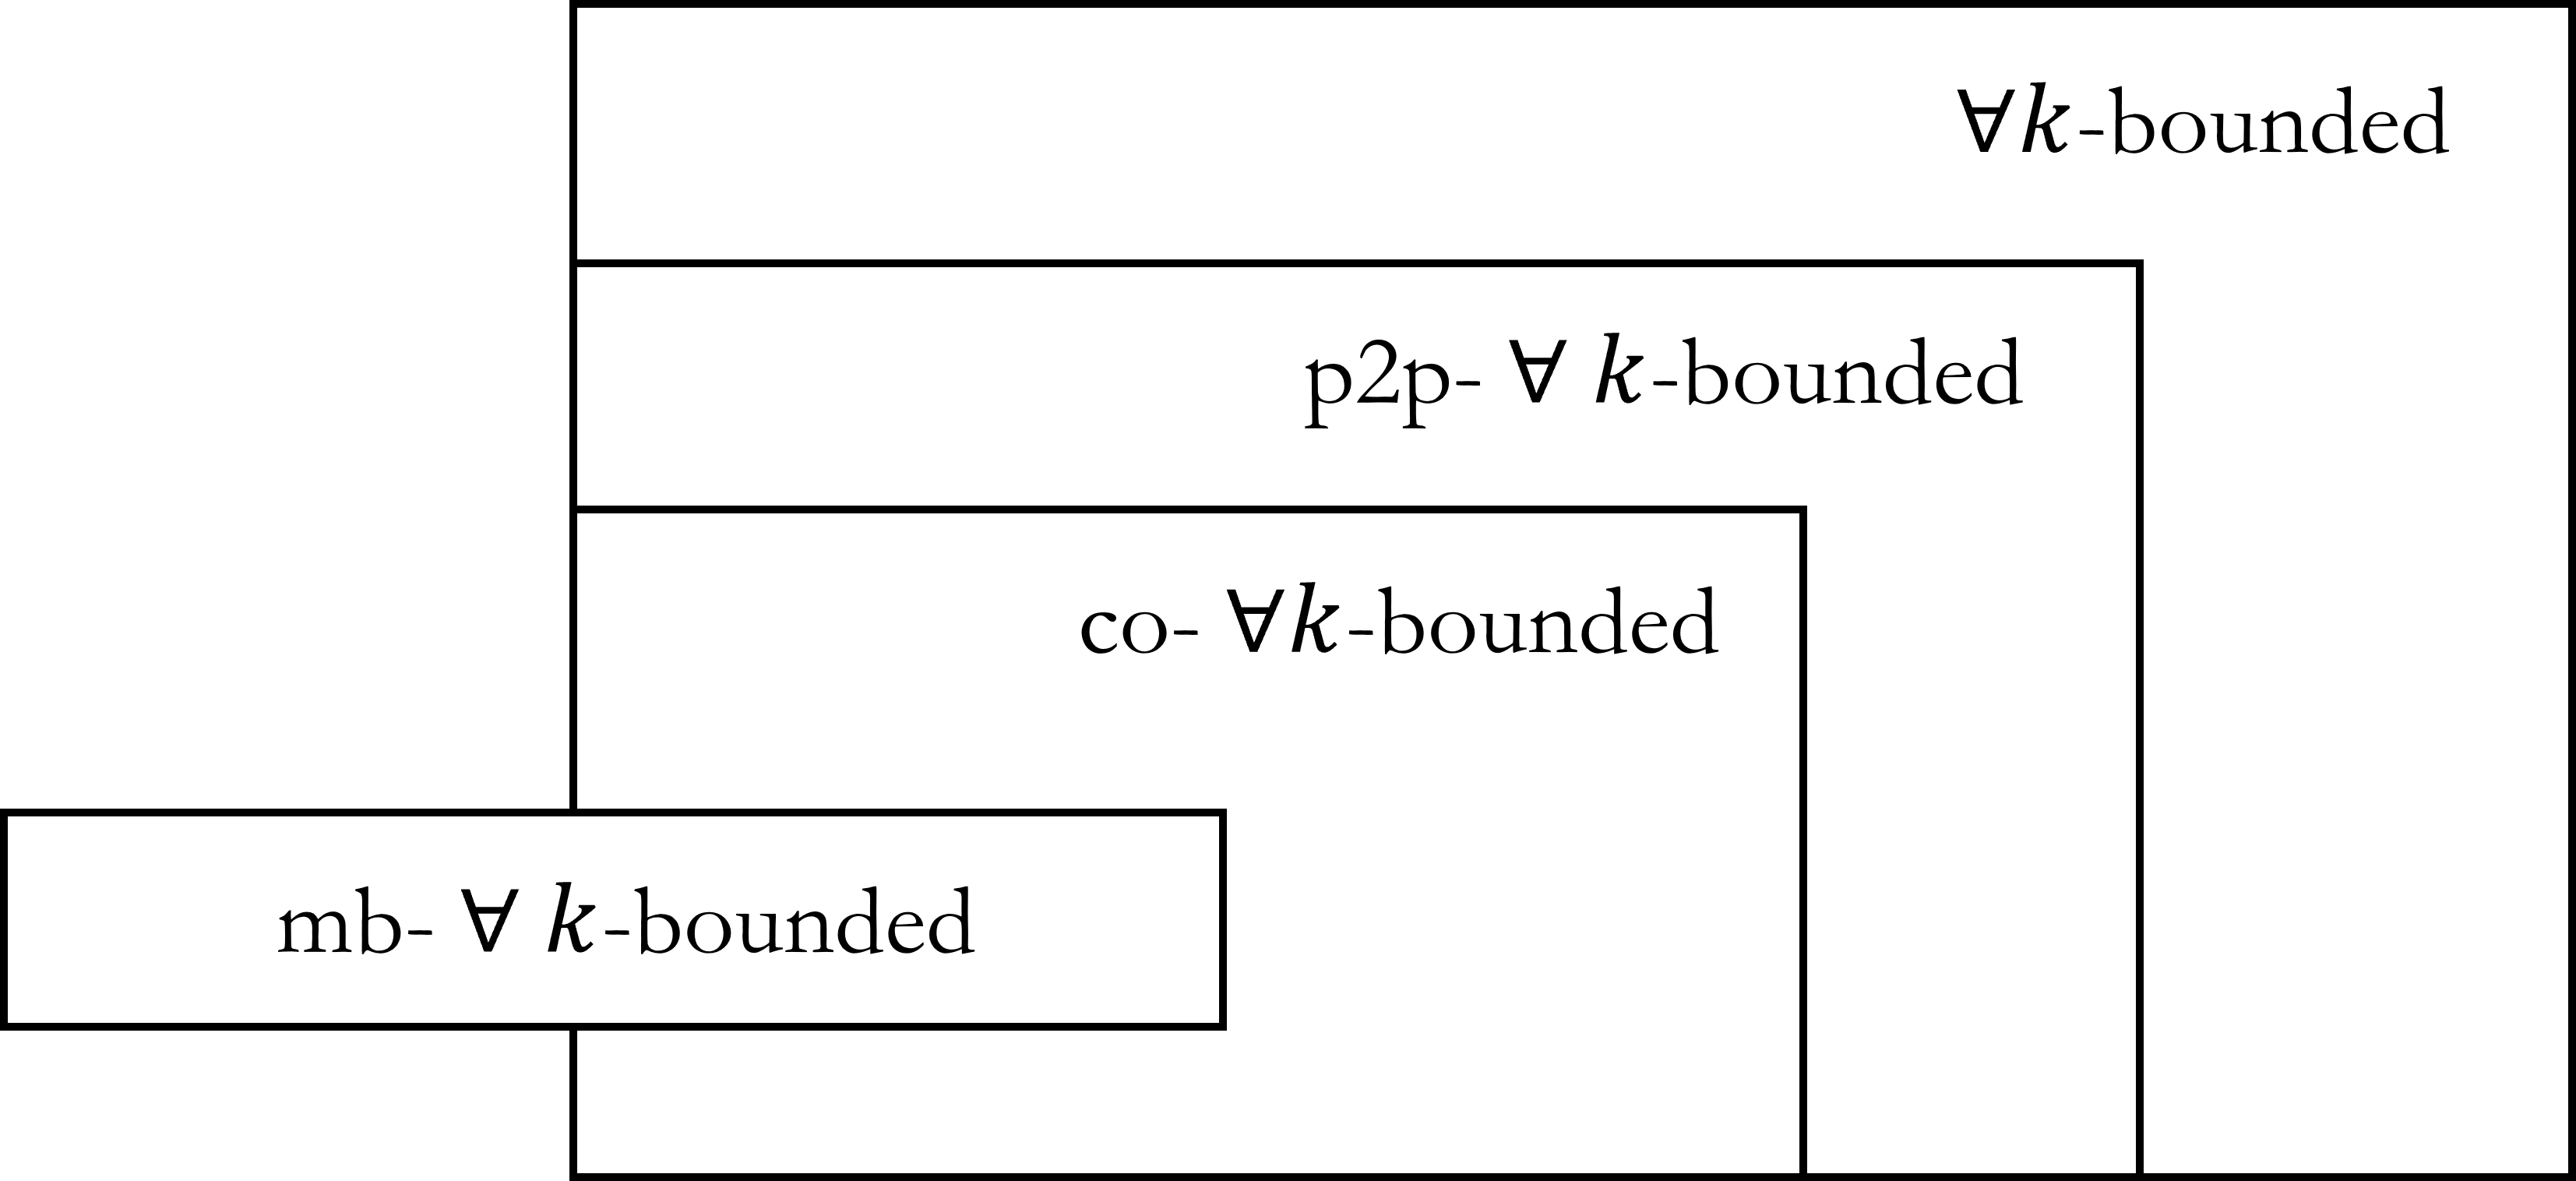
\includegraphics[width=8cm]{uni_k_hierarchy.png}
% 	\caption{The relation between different variants of universally $k$-bounded MSCs, given a $k \in \N$.}
% 	\label{fig:uk_hierarchy}
% \end{figure}

\subsubsection{MSO-definability}

In this section, we will investigate the MSO-definability of all the variants of universally $k$-bounded MSCs that we introduced.

In \cite{DBLP:conf/fossacs/LohreyM02}, it is shown that an MSC $\msc$ is universally $k$-bounded if and only if $\relb \;\subseteq\; \le_\msc$. In other words, $r \relb s \Rightarrow r \le_\msc s$ for any two events $r$ and $s$. This is equivalent to saying that every linearization $\linrel$ of $\msc$ respects the $\relb$ relation, since $\relb \;\subseteq\; \le_\msc \;\subseteq\; \linrel$. We already showed that $\relb$ is MSO-definable. The MSO formula that defines universally $k$-bounded  MSCs can be written as
\[ \asUkformula = \neg \exists r.\exists s.(r \relb s \wedge \neg(r \le_\msc s)) \]
Causally ordered and \pp universally $k$-bounded MSCs are clearly MSO-definable by definition, since we already showed that \pp MSCs, causally ordered MSCs, and universally $k$-bounded MSCs are all MSO-definable. To show MSO-definability of mailbox universally $k$-bounded MSCs we first prove the following property.

\begin{proposition}\label{prop:mb_ukb_alt}
	An MSC $\msc$ is mailbox universally $k$-bounded if and only if $\relb \;\subseteq\; \preceq_\msc$.
\end{proposition}
\begin{proof}
	Consider an MSC $\msc$ and a $k \in \N$.\newline
	($\Leftarrow$) Suppose $\relb \;\subseteq\; \preceq_\msc$. For every mailbox linearization $\mblinrel$ of $\msc$ we have that $\preceq_\msc \;\subseteq\; \mblinrel$. This implies $\relb \;\subseteq\; \mblinrel$, that is to say every mailbox linearization is $k$-bounded.\newline
	($\Rightarrow$) Suppose $\msc$ is a mailbox universally $k$-bounded MSC. By definition, every mailbox linearization $\mblinrel$ of $\msc$ is $k$-bounded, i.e. $\relb \;\subseteq\; \mblinrel$, and we have $\preceq_\msc \;\subseteq\; \mblinrel$, according to the definition of mailbox linearization. Moreover, we also know that $\preceq_\msc \cup \relb$ is acyclic, since $\msc$ is existentially $k$-bounded\footnote{Every mailbox universally $k$-bounded MSC is also a mailbox existentially $k$-bounded MSC by definition.}. Suppose now, by contradiction, that $\relb \;\nsubseteq\; \preceq_\msc$. Thus, there must be at least two events $r$ and $s$ such that $r \relb s$ and $r \npreceq_\msc s$; we also have $s \npreceq_\msc r$ because of the acyclicity of $\preceq_\msc \cup \relb$ (we cannot have the cycle $r \relb s \preceq_\msc r$). Consider a mailbox linearization $\mblinrel$  of $\msc$, such that $s \mblinrel r$. Note that such a mailbox linearization always exists, since $r$ and $s$ are incomparable w.r.t. the partial order $\preceq_\msc$ (i.e. $s \npreceq_\msc r$)\footnote{If two elements $a$ and $b$ of a set are incomparable w.r.t. a partial order $\le$, it is always possible to find a total order of the elements (that respects $\le$) where $a$ comes before $b$, or viceversa.}. This mailbox linearization does not respect $\relb$ (because we have $s \mblinrel r$ and $r \relb s$), so it is not $k$-bounded. This is a contradiction, since we assumed that $\msc$ was a mailbox universally $k$-bounded MSC. It has to be that $\relb \subseteq \preceq_\msc$.
\end{proof}

Using Proposition~\ref{prop:mb_ukb_alt}, we can now easily write the MSO formula that defines mailbox universally $k$-bounded MSCs as
\[ \mbUkformula = \neg \exists r.\exists s.(r \relb s \wedge \neg(r \preceq_\msc s)) \]

\subsubsection{Special treewidth}

All the variants of universally $k$-bounded MSCs that we presented have a bounded special treewidth. This directly follows from the STW-boundness of the existential counterparts, since every universally $k$-bounded MSC is existentially $k$-bounded by definition.
